%File: formatting-instructions-latex-2024.tex
%release 2024.0
\documentclass[letterpaper]{article} % DO NOT CHANGE THIS
\usepackage{aaai24}  % DO NOT CHANGE THIS
\usepackage{times}  % DO NOT CHANGE THIS
\usepackage{helvet}  % DO NOT CHANGE THIS
\usepackage{courier}  % DO NOT CHANGE THIS
\usepackage[hyphens]{url}  % DO NOT CHANGE THIS
\usepackage{graphicx} % DO NOT CHANGE THIS
\urlstyle{rm} % DO NOT CHANGE THIS
\def\UrlFont{\rm}  % DO NOT CHANGE THIS
\usepackage{natbib}  % DO NOT CHANGE THIS AND DO NOT ADD ANY OPTIONS TO IT
\usepackage{caption} % DO NOT CHANGE THIS AND DO NOT ADD ANY OPTIONS TO IT
\frenchspacing  % DO NOT CHANGE THIS
\setlength{\pdfpagewidth}{8.5in}  % DO NOT CHANGE THIS
\setlength{\pdfpageheight}{11in}  % DO NOT CHANGE THIS
%
% These are recommended to typeset algorithms but not required. See the subsubsection on algorithms. Remove them if you don't have algorithms in your paper.
\usepackage{algorithm}
\usepackage{algorithmic}

%
% These are are recommended to typeset listings but not required. See the subsubsection on listing. Remove this block if you don't have listings in your paper.
\usepackage{newfloat}
\usepackage{listings}
\DeclareCaptionStyle{ruled}{labelfont=normalfont,labelsep=colon,strut=off} % DO NOT CHANGE THIS
\lstset{%
	basicstyle={\footnotesize\ttfamily},% footnotesize acceptable for monospace
	numbers=left,numberstyle=\footnotesize,xleftmargin=2em,% show line numbers, remove this entire line if you don't want the numbers.
	aboveskip=0pt,belowskip=0pt,%
	showstringspaces=false,tabsize=2,breaklines=true}
\floatstyle{ruled}
\newfloat{listing}{tb}{lst}{}
\floatname{listing}{Listing}
%
% Keep the \pdfinfo as shown here. There's no need
% for you to add the /Title and /Author tags.

% DISALLOWED PACKAGES
% \usepackage{authblk} -- This package is specifically forbidden
% \usepackage{balance} -- This package is specifically forbidden
% \usepackage{color (if used in text)
% \usepackage{CJK} -- This package is specifically forbidden
% \usepackage{float} -- This package is specifically forbidden
% \usepackage{flushend} -- This package is specifically forbidden
% \usepackage{fontenc} -- This package is specifically forbidden
% \usepackage{fullpage} -- This package is specifically forbidden
% \usepackage{geometry} -- This package is specifically forbidden
% \usepackage{grffile} -- This package is specifically forbidden
% \usepackage{hyperref} -- This package is specifically forbidden
% \usepackage{navigator} -- This package is specifically forbidden
% (or any other package that embeds links such as navigator or hyperref)
% \indentfirst} -- This package is specifically forbidden
% \layout} -- This package is specifically forbidden
% \multicol} -- This package is specifically forbidden
% \nameref} -- This package is specifically forbidden
% \usepackage{savetrees} -- This package is specifically forbidden
% \usepackage{setspace} -- This package is specifically forbidden
% \usepackage{stfloats} -- This package is specifically forbidden
% \usepackage{tabu} -- This package is specifically forbidden
% \usepackage{titlesec} -- This package is specifically forbidden
% \usepackage{tocbibind} -- This package is specifically forbidden
% \usepackage{ulem} -- This package is specifically forbidden
% \usepackage{wrapfig} -- This package is specifically forbidden
% DISALLOWED COMMANDS
% \nocopyright -- Your paper will not be published if you use this command
% \addtolength -- This command may not be used
% \balance -- This command may not be used
% \baselinestretch -- Your paper will not be published if you use this command
% \clearpage -- No page breaks of any kind may be used for the final version of your paper
% \columnsep -- This command may not be used
% % \newpage -- No page breaks of any kind may be used for the final version of your paper
% \pagebreak -- No page breaks of any kind may be used for the final version of your paperr
% \pagestyle -- This command may not be used
% \tiny -- This is not an acceptable font size.
% \vspace{- -- No negative value may be used in proximity of a caption, figure, table, section, subsection, subsubsection, or reference
% \vskip{- -- No negative value may be used to alter spacing above or below a caption, figure, table, section, subsection, subsubsection, or reference
\setcounter{secnumdepth}{0} %May be changed to 1 or 2 if section numbers are desired.

% The file aaai24.sty is the style file for AAAI Press
% proceedings, working notes, and technical reports.
%

% Title

% Your title must be in mixed case, not sentence case.
% That means all verbs (including short verbs like be, is, using,and go),
% nouns, adverbs, adjectives should be capitalized, including both words in hyphenated terms, while
% articles, conjunctions, and prepositions are lower case unless they
% directly follow a colon or long dash
% \title{A Dataset and Scalable, Transparent, Online Open Learner Models for Recommending Educational Videos on Artificial Intelligence}
\title{A Toolbox for Modelling Engagement with Educational Videos}


%\title{A Dataset and Scalable, Transparent, Online Learner Models for Engagement Modelling with Educational Videos on Artificial Intelligence}
\author{
Yuxiang Qiu\equalcontrib,
Karim Djemili\equalcontrib,
Denis Elezi\equalcontrib,
Aaneel Shalman Srazali\equalcontrib,
Mar\'ia P\'erez-Ortiz,
Emine Yilmaz,
John Shawe-Taylor and
Sahan Bulathwela
}

\affiliations{
Department of Computer Science, University College London \\
Gower Street, London WC1E 6BT, UK\\
m.bulathwela@ucl.ac.uk
}


% REMOVE THIS: bibentry
% This is only needed to show inline citations in the guidelines document. You should not need it and can safely delete it.
\usepackage{bibentry}
% END REMOVE bibentry

\begin{document}

\maketitle

\begin{abstract}
With the advancement and utility of Artificial Intelligence (AI), personalising education to a global population could be a cornerstone of new educational systems in the future. This work presents the \emph{PEEKC} dataset and the \emph{TrueLearn} Python library, which contains a dataset and a series of online learner state models that are essential to facilitate research on learner engagement modelling. %with AI-related educational Videos.
TrueLearn family of models was designed following the "open learner" concept, using humanly-intuitive user representations.
This family of scalable, online models also help
% For the sake of interpretability and putting the user in control, the TrueLearn library also contains different representations to help
end-users visualise the learner models, which may in the future facilitate user interaction with their models/recommenders.
% Together with the library, we include a previously publicly released implicit feedback educational dataset with evaluation metrics to measure the performance of the models.
The extensive documentation and coding examples make the library highly accessible to both machine learning developers and educational data mining and learning analytics practitioners.
The experiments show the utility of both the dataset and the library with predictive performance significantly exceeding comparative baseline models. The dataset contains a large amount of AI-related educational videos, which are of interest for building and validating AI-specific educational recommenders.
\end{abstract}

\section{Introduction}

It has been shown that personalised one-on-one learning could lead to improving learning gains by two standard deviations \cite{Bloom84}.
With this goal in sight, and the ambition to democratise education to a world population,
we require responsible intelligent systems that can bring scalable, personalised and governable models to a mass of learners \cite{democratise2021}.
% Up until recently, the go-to solution for scaling education has been
Intelligent Tutoring Systems (ITS), the go-to solution, is practical for courses with a limited number of learning materials and heavily relies on testing users for knowledge. However, today's world has access to 100,000s of rich educational videos, PDFs and podcasts that can be matched to a global population of lifelong learners.
Educational recommenders have the opportunity to
% go one step further,
leverage implicit interaction signals (such as clicks and watch time) to personalise and support learning for informal lifelong learners \cite{bulathwela2022sus}. Furthermore, {the scarcity of publicly available datasets of learners in the wild engaging with educational materials} is a major deterrent to creating scalable educational recommenders.
% This is exactly the focus of the models in this library, aiming to make such approaches more accessible, as openly available learner models and datasets are currently scarce, while they could bring great opportunities in education.

The contributions of this paper are two-fold. Firstly, we create and release to the public the \textbf{P}ersonalised \textbf{E}ducational \textbf{E}ngagement linked to \textbf{K}nowledge \textbf{C}omponents (PEEKC) dataset, with more than 20,000 informal learners watching educational videos in an in-the-wild setting (i.e. learning informally). The videos in the PEEKC dataset majorly contain concepts related to Artificial Intelligence (AI) and Machine Learning (ML) making it a valuable resource for AI-assisted education on these topics. Secondly, we develop and release \emph{TrueLearn},
% \footnote{Documentation available at \url{https://truelearn.readthedocs.io/en/latest/}}
an open-source Python library packaging state-of-the-art Bayesian models and visualisation tools for leveraging scalable, online learning, transparent learner models. The library contains different components that will enable i) creating content representations of learning resources ii) managing user/learner states, iii) modelling the state evolution of learners using interactions and iv) evaluating engagement predictions. This work uses the PEEKC dataset to empirically demonstrate the predictive capabilities of the different models within the TrueLearn library.

% This work introduces \emph{TrueLearn}\footnote{Documentation available at \url{https://truelearn.readthedocs.io/en/latest/}}, an open-source Python library that packages state-of-the-art online recommendation models, datasets and visualisation tools. Among a wide variety of use cases, it can be used e.g. to incorporate a personalisation component in an e-learning platform (e.g. YouTube and EdX) that can capture user clicks and watch time (of videos/lectures) by estimating the potential engagement of a learner with a learning resource, modelling relevant variables such as background knowledge, interest and novelty. The library contains different components that will enable i) creating content representations of learning resources ii) managing user/learner states, iii) modelling the state evolution of learners using interactions and iv) evaluating engagement predictions. Requiring minimal data, its design offers a transparent solution that respects the privacy of its users and enables user interaction. The development of the TrueLearn library aims to provide both the research and developer communities with the opportunity to use the TrueLearn family of models.
% The paper describes the development process and experiments that demonstrate the utility of this package to the educational data mining community and beyond.


% While the motivation for TrueLearn stems from education, the models are applicable to a wide variety of applications that relate to informational recommendations and to model engagement in tasks in which human learning is involved. Additionally, note that the models included are suitable both for implicit and explicit feedback. In our experiments, we used a dataset of videolectures watch patterns, which we use as a proxy for learner engagement, but the same models could be applicable if learners also provided e.g. explicit feedback on the difficulty of the learning material.

\section{Related Work}

The scarcity of publicly available datasets
% \cite{mltidbits}
for predicting learner engagement with educational videos constrains the growth of the personalisation of AI education. PEEKC is the first and largest learner video engagement dataset publicly released with humanly interpretable Wikipedia concepts and the concept coverage associated with the video lecture fragments.
Next, we present relevant works to i) the PEEKC dataset (not only related datasets but also research on the approaches that were used to generate it, e.g. Wikification) and ii) our novel machine learning library.
% We have researched related work on learner models and how to design usable machine learning libraries to make decisions regarding the design of the TrueLearn library. This section reviews these works and their influence on the development of the library.

\subsection{Related Datasets}

% The datasets related to PEEKC are for \emph{knowledge tracing} domain\cite{corbett1994knowledge,deep_kt} which focuses on modelling knowledge/skill mastery of learners based on test taking. This approach, as discussed in Section \ref{lit_review}, is much more explicit and effort intense than inferring it using implicit feedback (e.g. watched patterns of educational videos).
\emph{Knowledge Tracing} \cite{corbett1994knowledge,deep_kt}, focussing on modelling knowledge/skill mastery of learners based on test-taking is the most active research area in the learner modelling domain. ASSISTments data \cite{assistments_data}, which records learners solving mathematics problems, is often used in literature while this data is mathematics education focused.
% Majority of related datasets such as ASSISTments data \cite{assistments_data}, ednet that records a series of learners solving tests in an ITS platform. These datasets are heavily biased towards mathematics knowledge as the ASSISTments tool was used for mathematics education from the beginning \cite{assist_math1,mcguire2017counterintuitive}.
Additionally,
% A few publicly available datasets to solve knowledge tracing problem exist. They include mathematics ASSISTments\footnote{\url{http://www.assistmentstestbed.org/}}\cite{assistmentHurstC18,walkington2019effect},
problem-solving interactions \cite{choi2020ednet}, multiple choice question answering \cite{wang2020diagnostic,wang2021educational} datasets exist publicly while none of them includes implicit feedback related to consuming educational videos.
% , all of which are noteworthy although they do not focus on implicit feedback and engagement.
MOOCCube dataset contains a spectrum of different statistics relating to learner-MOOC interactions including implicit and explicit test-taking activity \cite{yu2020mooccube}. Although this dataset may contain data that can be used to predict learner engagement which has been used for course recommendation \cite{deng2023knowledge}, the pre-organisation of courses takes away the in-the-wild choices learners make in choosing videos/fragments to watch while the courses in MOOCCube are not limited to AI. On the contrary, PEEKC dataset presents over 20,000 informal learners watching AI-related videos with fragment-level annotation of videos providing more granularity at a time segment/fragment level information retrieval is gaining interest \cite{yu2020spotify}.

\subsection{Extracting Knowledge Components}

ITSs often rely on expert labelling of the \textbf{Knowledge Components (KCs)} \cite{assistments_data}
% (sometimes also for the hierarchy of knowledge\cite{bauman2018recommending} and defining a Q-matrix\cite{tatsuoka1983rule})
, which is time-consuming and not scalable. Unsupervised learning approaches
% , Latent Semantic Analysis (LSA)\cite{dumais2004latent} and other probabilistic approaches\cite{hofmann2013probabilistic,liang2019collaborative}
are also potential candidates.
{Latent Dirichlet Allocation (LDA) has widely been used to extract topic metadata from different types of text data including course syllabuses \cite{Apaza2014OnlineCR}. However, unsupervised approaches such as LDA suffer from complex hyper-parameter tuning \cite{PANICHELLA2021106411}} and limited interpretability of \emph{latent} KCs, creating gaps in transparency. % Since then, entity linking has shown great promise towards this goal \cite{wikifier}.
\emph{Wikification}, a form of entity linking \cite{wikifier}
% which automatically links Wikipedia pages to text,
has shown promise for automatically capturing the KCs covered in an educational resource \cite{truelearn}. This technology provides \emph{automatic}, \emph{humanly-intuitive (symbolic)} representations from Wikipedia, representing \emph{up-to-date knowledge} about \emph{many domains}.
% Wikipedia, being one of the largest encyclopedias in the world, evolves with time due to the contributor population that constantly updates it.


% Although majority of studies in the field focus on recommending content items that are relevant to a learner,
The possibility of recommending parts of items (contrary to an entire video or podcast) is also a fruitful research direction explored lately. From proximity-aware information retrieval
% that exploits the positional structure of tokens
\cite{schenkel2007efficient} to segmenting videos to build tables of contents \cite{videoken}, this goal has been under active research. Breaking informational videos into fragments has also shown promise in efficient previewing \cite{chen2018temporally} and enabling non-linear consumption of videos \cite{non_lin}. Recent proposals such as TrueLearn \cite{truelearn} demonstrate the potential of using fragment recommendation in education. %While personalisation models are being proposed for recommendation, publishing datasets will enable the community to join hands in advancing this research direction.
% For these experiments, we created video parts of 5,000 characters (5 minutes) in the fragmentation process. This allows the e-learning system to have video fragments that contain a satisfactory amount of knowledge while keeping the video fragment length at a favourable value in terms of retaining viewer engagement \cite{Guo_vid_prod}.
% While TrueLearn Novel demonstrates promise, we strongly believe that availability of such a dataset to the public is critical in pushing the frontiers of research in (fragment-based) educational recommendation. PEEKC dataset addresses this need.
Due to these reasons, we use Wikification \cite{wikifier} to generate KCs that are included in each video fragment covered by the PEEKC dataset.



% Although previous work based on popular video repositories such as edX\cite{Guo_vid_prod}, Khan Academy\cite{khan_bigdata}, VideoLectures\cite{truelearn,trueeducation} and YouTube\cite{beyondviews,Covington2016} has evidenced the existence of datasets that include implicit engagement signals, these datasets are never made public due to their proprietary nature.
% The scarcity of large scale publicly available datasets for predicting learner engagement with educational videos constrain the growth of the field.

% \subsection{Item Response Theory and Knowledge Tracing}

% % As mentioned in \textit{A Family of Bayesian Algorithms to Match Lifelong Learners to Open Educational Resource}
% Item Response Theory (IRT) focuses on designing, analysing and scoring ability tests by modelling learner’s knowledge and question difficulty, without considering changes in knowledge over time. The simplest of IRT, the Rasch model \cite{Rasch1960}, computes the probability of scoring a correct answer as a function of the learner’s skill $\theta_l$ and the difficulty of the question/resource $d_r$:
% \begin{equation}
% P(correct\:answer|\theta_l, d_r) = f(\theta_l - d_r)
% \end{equation}
% where $f$ is usually a logistic function. TrueSkill model extends IRT to model the skill of multiple users playing a video game \cite{trueskill}. The TrueLearn models implemented in this work extend TrueSkill for learner engagement prediction.

% % By replacing the learner and resource with two different players, we obtain the Elo rating system \cite{elo}, commonly used to rank chess players based on their game outcomes. The TrueSkill algorithm \cite{trueskill} takes this a step further, allowing entire teams of players to compete and adding a dynamic component to update player skills over time.
% % The original TrueLearn algorithms \cite{truelearn}, which model learning as a game between a team composed of the knowledge components (KCs) of the learner and an opposing team made up of the KCs covered by the learning resource, use TrueSkill to update the learner's skill based on the outcome of the match. TrueSkill serves as the foundation of TrueLearn and as such acts as a fundamental dependency in the library.

% % \subsection{Knowledge Tracing (KT) and pyBKT}
% An alternative to IRT for modelling learning is Knowledge Tracing (KT) \cite{corbett1994knowledge}. Unlike IRT, KT model does not consider question difficulty but instead estimates knowledge acquisition as a function of practice opportunities. Several Bayesian KT (BKT) algorithms that extend the original KT model have been proposed in the literature. The pyBKT library, a Python library of KT models provides a clear Application Programming Interface advocating the separation of data generation, model fitting and prediction functions \cite{pybkt}. However, conventional KT models do not train using online learning, introducing challenges when scaling to real-time scenarios with a large number of users learning over a long period of time.
% While online formulations of KT exist \cite{bishopsnewbook}, they are not included in openly released code libraries.
% , also ensures the models' correctness and computational efficiency through testing . pyBKT is of relevance to this project since, by bundling BKT algorithms into an open-source package, it makes them accessible to other researchers and developers, which is precisely what TrueLearn aims to do with the existing TrueLearn algorithms.

\subsection{Designing a Machine Learning Library}

% if needed, this can be removed
% we only need to change the first sentence of the next paragraph
% While many design principles \cite{martin2000design} and patterns \cite{gamma1995design} have been proposed to address the problem of designing scalable and maintainable software, ...
To design a user-friendly, easy-to-use, and scalable library, commonly used yet, bad design practices, such as rigidity, fragility, immobility and viscosity should be avoided \cite{martin2000design,piccioni2013empirical}.
% refers to the tendency for software to be difficult to change. Fragility is the tendency for software to break once it has been updated. Immobility is the inability to reuse code within or across projects. Viscosity refers to the difficulty of retaining the original design when changes to the software are required.
Many design principles are proposed to overcome these issues \cite{gamma1995design}. Many data scientists also prefer usable (adhering to known patterns), well-documented and intuitive libraries \cite{nadi2023selecting}.
% For example, the strategy pattern makes code more flexible and reusable by deferring algorithm selection to runtime; the iterator pattern encourages the use of iterators to traverse and access data in containers, thus decoupling algorithms from data and resulting in easier software updates and code reuse.
Besides these, designing a machine learning library entails overcoming additional challenges (e.g. data, pre-processing, models, etc.).
% When designing a machine learning library, we also need to account for unique challenges (e.g. incorporating data, pre-processing, models etc.). A great example a well-designed machine learning library that has been taken up by both industry and academia recently is \texttt{scikit-learn}.
% While the above patterns solve many of the problems of designing software, designing machine learning libraries presents unique challenges because it focuses more on models, data, parameters, and hyperparameters. This requires the library designers to consider how users set the hyperparameters of the model, prepare data for the training process, train the model based on the data, and use the trained model to accomplish their tasks.
Scikit-learn \cite{pedregosa2011scikit} proposes consistency, inspection, sensible defaults and good interface design (estimators and predictors) for building a scalable and user-friendly machine learning library. Consistency of the code interfaces significantly reduces the learning cost for users while inspection exposes relevant model parameters and public attributes to the user with easy access \cite{buitinck2013api}.
% emphasises the importance of establishing a shared and consistent interface across different machine learning models, as this reduces the learning cost of the library. Inspection is concerned with exposing the model's parameters and hyperparameters as public attributes, which makes it easier for users to access the internal states of the model. Sensible defaults ensure that the model behaves reasonably well with the default values.
% The estimator and predictor interfaces in scikit-learn reflect how the library implements these general guidelines.
The estimator interface specifies a \verb|fit| function to provide a consistent interface to the training model and exposes the \verb|coef_| attribute to facilitate the inspection of the internal state of the model. The predictor interface specifies the \verb|predict| and \verb|predict_proba| functions as methods for utilising the trained model. PyBKT, a Python-based library that implements knowledge tracing and item response theory-based learner models, also follow the same interfacing practices where function names \verb|fit| and \verb|evaluate| are used to train and predict \cite{psych5030050}.
Due to the time-tested and consistent design decisions that have succeeded in scikit-learn and pyBKT, we utilise the same functions to interact with the learner models in the TrueLearn library.

% Because of the concept of duck typing in Python, others' model implementations can interoperate with scikit-learn (e.g., developers can plug them into scikit-learn's grid search) without being forced to inherit the above interfaces. This makes scikit-learn extensible and encourages users to reuse code. However, the use of duck typing makes it difficult to perform static program analysis \cite{milojkovic2017duck}, thus postponing the discovery of incorrect implementations until runtime and increasing the likelihood of software bugs \cite{chen2020typing}. Therefore, in our work, we tend to take a hybrid approach, utilising type annotations \cite{pep484} throughout the codebase while allowing the use of static duck types supported by the \texttt{Protocol} class \cite{pep544}. Compared to traditional duck typing, static duck typing allows the library implementer to represent the requirement for parameters of a method explicitly but also does not force the user to inherit any class, making it easier for users to understand the intent of the method and helping static type checkers to analyse the code \cite{pep544}.

\subsection{Learner Modelling}

Personalised learning mainly revolves around Knowledge Tracing (KT) \cite{psych5030050} and Item-Response Theory (IRT) \cite{Rasch1960} based models that use KCs in exercises to predict test success. However, these models focus on test-taking (modelling short sequences of exercise answering events) rather than consuming learning materials such as video watching. Conventional KT and IRT models do not support online learning posing scale challenges in lifelong learning cases (while online counterparts exist \cite{bishopsnewbook}). More recently, deep-KT \cite{deep_kt} has shown promise in superior performance. However, deep-KT models are data-hungry and lack interpretability, making them less favourable for lifelong learning, where the model needs to learn usable parameters with minimal data. Furthermore, recent studies have questioned the superior performance of deep-KT models in comparison to traditional models \cite{Schmucker_Wang_Hu_Mitchell_2022}. Due to these reasons, we scope out batch/deep learning models and focus on data-efficient online models.

The TrueLearn family of online Bayesian learner models uses implicit feedback from learners to recover their learning state \cite{truelearn}. Models that capture learners' interests, knowledge, and novelty are proposed in prior work with methods to combine them as interpretable ensembles that can account for these factors simultaneously \cite{bulathwela2022sus}.
While being data efficient and privacy-preserving by design
(exclusively using individual learner's interactions)
,
TrueLearn models generate humanly intuitive learner representations inspired by Open Learner Models (OLM).
% An open learner model is a learner model that has been made accessible to the learner it represents or to other users (e.g. teachers, parents) .
This involves generating visualisations that will communicate information about learner state, promoting learner reflection by aiding learners in planning and monitoring their learning \cite{openlearnermodels}.
% Open learner models come with definite advantages, such as promoting learner reflection by aiding learners in planning and monitoring their learning and allowing them to compare their knowledge to that of their peers \cite{openlearnermodels}.
OLMs also pose challenges, since all visual presentations may not be equally understood by a wide variety of end-users. Among many visualisations used to present learner knowledge state, user studies have shown that some visualisations are comparatively more user-friendly than others \cite{10.1007/978-3-319-98572-5_40,visualisationscomparison}. TrueLearn implements a set of tested visualisations that aid the communication and the interaction process.

Both deep KT and libraries such as pyBKT focus on predicting test-taking behaviour \cite{psych5030050} rather than how they would interact with an educational video. These libraries also focus on course-based learning settings where the number of KCs and learning items are limited in number. In these aspects, TrueLearn sets itself apart from the rest of the available libraries. The same reasons make TrueLearn valuable for MOOC platforms and educational video repositories that thrive to personalise videos for learning. In a world where a large number of educational videos are in circulation, we are unaware of a public, easy-to-use toolkit that can be used to incorporate educational video personalisation apart from our proposal, TrueLearn.


% As such, it was of great importance to select the visualisations forming the interface appropriately by considering their effectiveness in communicating information about the learner model, and their ease of understanding to ensure that all learners, regardless of their background, would be able to benefit from them. Research ranking visualisations on these two criteria already existed () and we referred to it when determining which visualisations our library would be able to generate.

\section{Problem Setting}

% \figurename{ \ref{fig:prob}} illustrates the educational recommendation scenario.
A learner $\ell$ in learner population $L$ interacting with a series of educational resources $S_\ell \subset \{r_1, \ldots, r_{R}\}$ where $r_x$ are \emph{fragments/parts} of an educational video $v$. The watch interactions happen over a period of $T$ time steps, $R$ being the total number of resources in the system.
In this system with a total $N$ unique knowledge components (KCs), resource $r_x$ is characterised by a set of top KCs or topics $K_{r_x} \subset \{1, \ldots, N \}$. We assume the presence $i_{r_x}$ of KC in resource $r_x$ and the degree $d_{r_x}\in \{ 0,1\}$ of KC coverage in the resource is observable.

% TODO: {-1, 1} or {0, 1}?
The key idea is to model the probability of engagement $e_{\ell, r_x}^{t} \in \{ 1, -1\}$ between learner $\ell$ and resource $r_x$ at time $t$ as a function of the learner interest $\theta^t_{\ell_{\texttt{I}}}$, knowledge $\theta^t_{\ell_{\texttt{NK}}}$ based on the top KCs covered $K_{r_x}$ using their presence $i_{r_x}$, and depth of topic coverage $d_{r_x}$.

% \begin{figure}[ht]
% %\vskip 0.2in
% \begin{center}
%     \centerline{\includegraphics[width=.75\columnwidth]{CameraReady/LaTeX/problem_setting.pdf}}
%     \caption{Visual illustration of the problem setting where learner $\ell$, with knowledge (that allows them to tackle novel content) $\theta_\texttt{NK}$ and interests $\theta_\texttt{I}$ is watching fragments of educational videos $r_x$ containing different knowledge components $K_{r_x}$ over time $t$.}
%     \label{fig:prob}
% \end{center}
% %\vskip -0.2in
% \end{figure}

\section{\texttt{PEEKC} Dataset}

In this section, we describe how the \textbf{P}ersonalised \textbf{E}ducational \textbf{E}ngagement linked to \textbf{K}nowledge \textbf{C}omponents (PEEKC) dataset is constructed. \figurename{ \ref{fig:peek_pipe}} (ii) outlines the overall process of creating the PEEKC dataset.
%\subsection{Data Source} \label{sec:data_source}
% PEEKC dataset is constructed using video metadata and learner activity data extracted from
PEEKC uses the data from VideoLectures.Net\footnote{\url{www.videolectures.net}} (VLN), a repository of scientific and educational video lectures. VLN repository records research talks and presentations from numerous academic venues (mainly AI and Computer Science). As the talks are recorded at peer-reviewed research venues, the lectures are reviewed and the material is controlled for the correctness of knowledge. Although most lectures consist of one video, some video lectures are broken into more videos (such as a long tutorial).
% First, all the lecture videos are transcribed.

% \figurename{ \ref{fig:vln_interface}} depicts the different components of the VLN user interface where a user engages with an educational video. Every lecture has a title, event details (e.g. conference venue, date, location etc.) and lecture meta data associated with it. Although most lectures consist of one video, some video lectures may contain more than one video as shown in \figurename{ \ref{fig:vln_interface}}.

% \begin{figure*}[ht]
% %\vskip 0.2in
% \begin{center}
%     \centerline{\includegraphics[width=.7\linewidth]{VLN.pdf}}
%     \caption{Screen layout of VideoLecture.Net website from which the data for PEEKC dataset was sourced. Every lecture can have one or more videos and is associated with metadata. The lecture transcripts are also available for processing.}
%     \label{fig:vln_interface}
% \end{center}
% %\vskip -0.2in
% \end{figure*}

\begin{figure*}[ht]
%\vskip 0.2in
\begin{center}
    \centerline{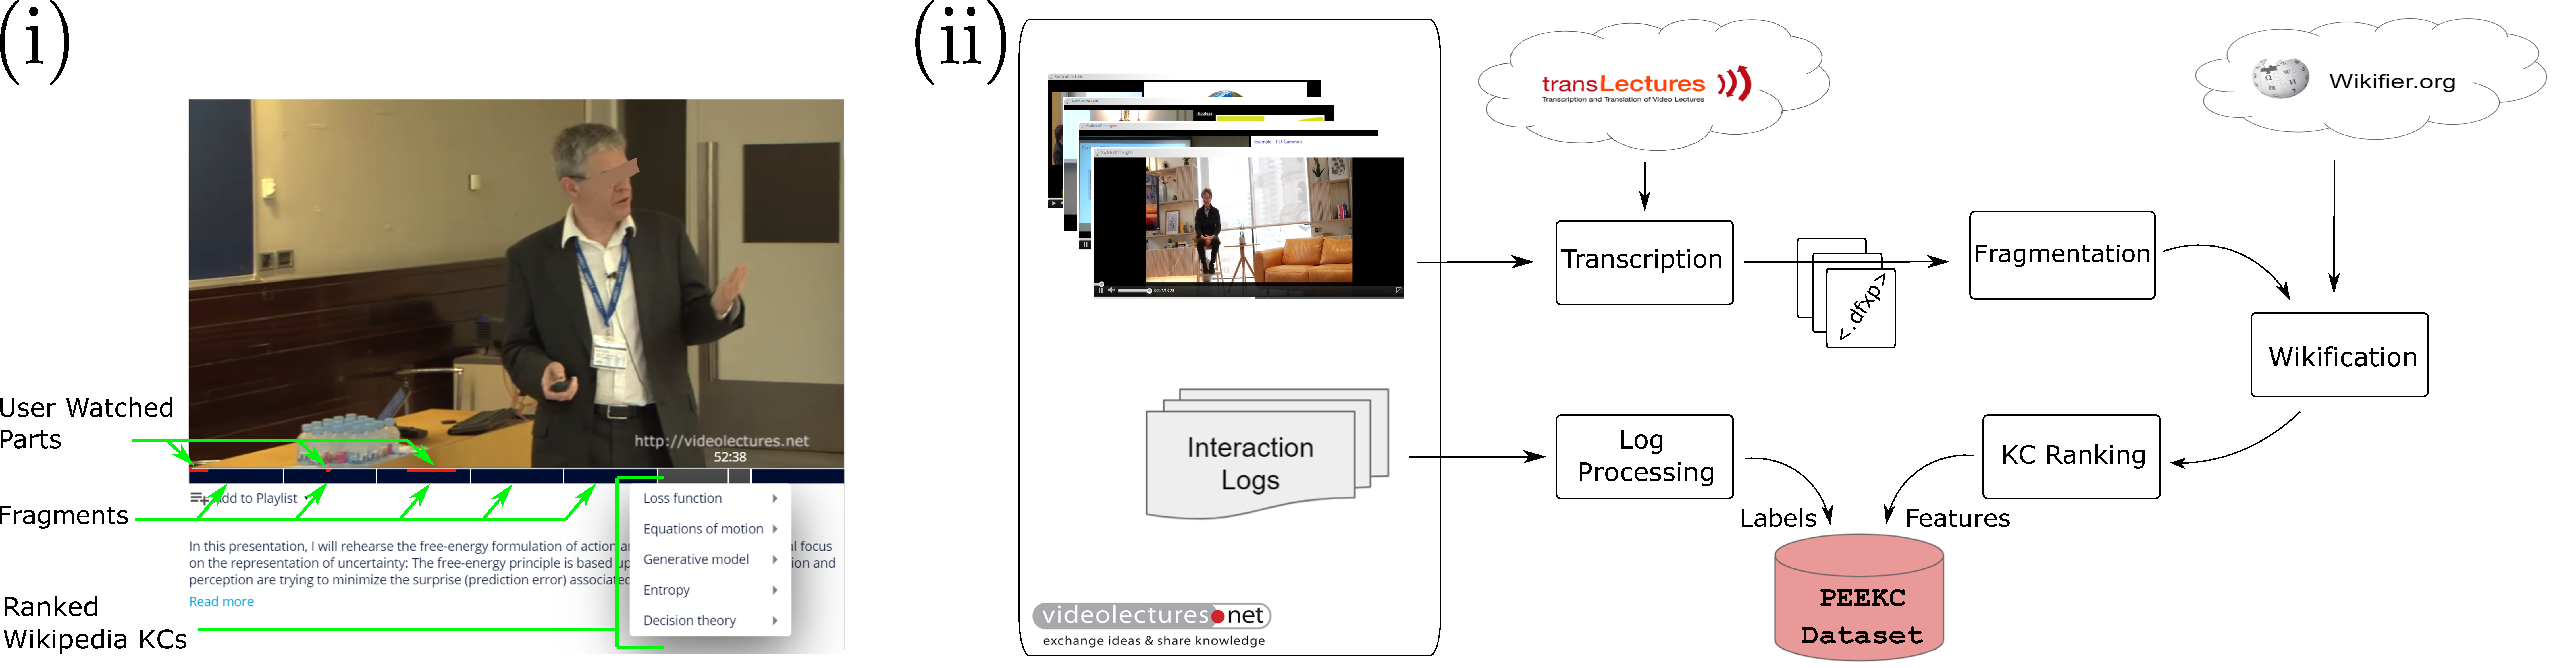
\includegraphics[width=.9\linewidth]{peek_data_pipe.pdf}}
    \caption{(i) Visual representation of the data items available in the PEEKC dataset where each video is broken into multiple, non-overlapping 5-minute fragments that are linked with ranked Wikipedia-based KCs and (ii) The flow chart presenting how the video data and the learner interaction logs from VLN repository are processed to create the PEEKC dataset.}
    \label{fig:peek_pipe}
\end{center}
%\vskip -0.2in
\end{figure*}

% \caption{(i) Visual representation of the data items available in the PEEKC dataset. Each video is broken into multiple, non-overlapping 5-minute fragments that are linked with ranked Wikipedia-based KCs. The watched parts of the video (in red) are used to create discrete engagement labels and (ii) The video data and the learner interaction logs from VLN repository are processed separately to create the Wikipedia-based KCs and also the discrete engagement signals that are published in PEEKC dataset.}

\subsection{Fragmenting Video Transcripts}

First, the videos in VLN repository are transcribed to its native language using the \emph{TransLectures} project\footnote{\url{www.translectures.eu}}. Then, the non-English lecture videos are translated into English as we will use English Wikipedia for entity linking.
% To model user interactions in a much more granular level we further break each video transcript into smaller parts.
Once the transcription/translation is complete, we partition the transcript of each video into multiple \emph{fragments} where each fragment covers approximately 5 minutes of lecture time (5000 characters).
% We believe 5 minutes is a good scoping measure as as such a time period allows having a satisfactory level of information contained in it.
Having 5-minute fragments allows us to break the contents of a video into a more granular level while making sure that there is sufficient amounts of information while keeping fragment length at a favourable value in terms of retaining viewer engagement \cite{Guo_vid_prod}.

\subsection{Wikification of Transcripts}
In order to identify the Knowledge Components (KCs) that are contained in different video fragments, we use Wikification \cite{wikifier}. This allows annotating learning materials with humanly interpretable KCs (Wikipedia concepts) at scale with minimum human-expert intervention. This setup will make sure that recommendation strategies built on this dataset will be technologically feasible for web-scale e-learning systems.
% Previous works have demonstrated the value of using Wikification in this task \cite{truelearn}. We restrict the dataset to English Wikipedia due to its richness.

% \begin{figure}[ht]
% %\vskip 0.2in
% \begin{center}
%     \centerline{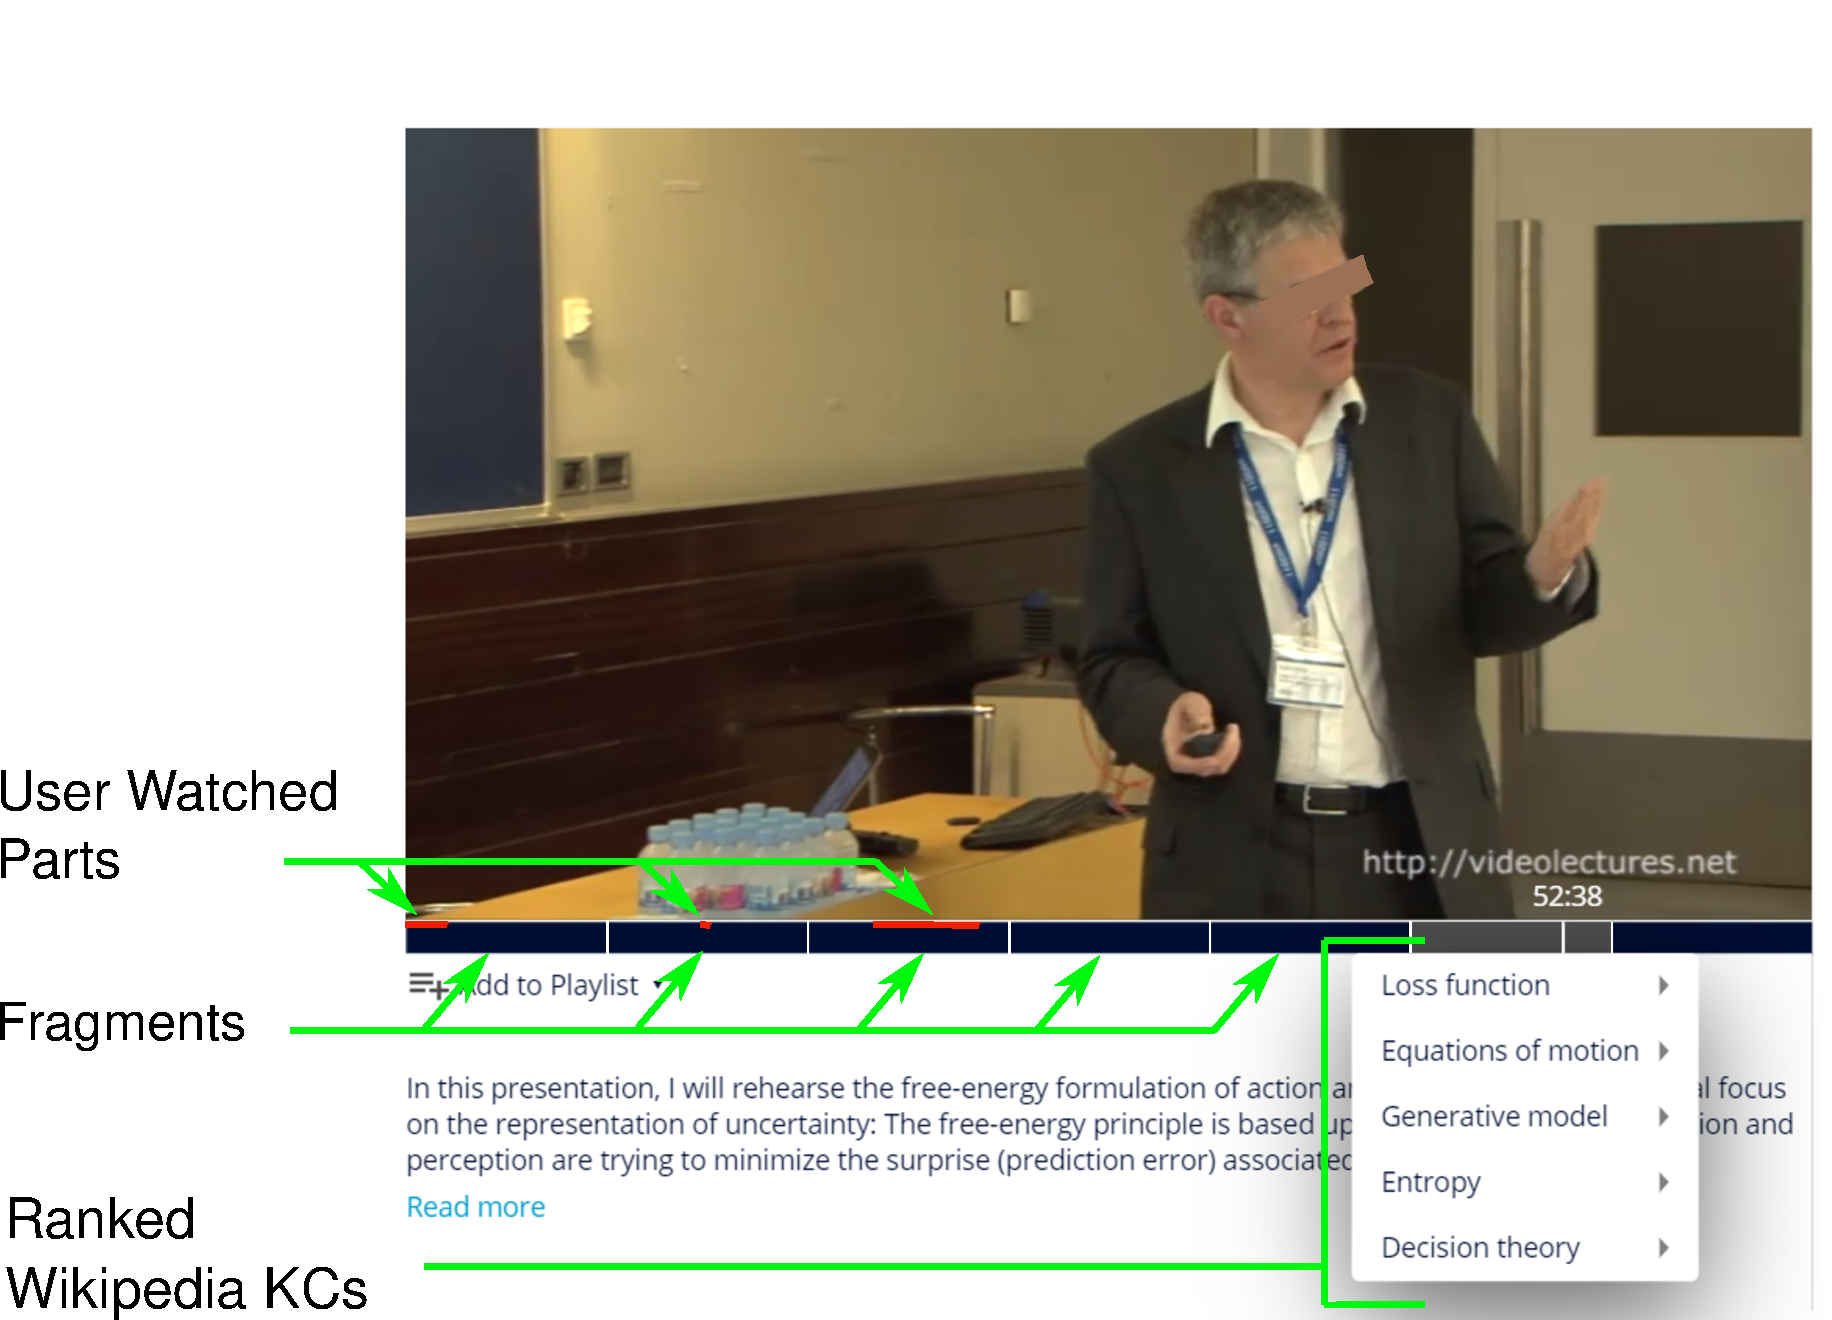
\includegraphics[width=\columnwidth]{CameraReady/LaTeX/fragments.pdf}}
%     \caption{Visual representation of the different data items available in the PEEKC dataset. Each video is broken into multiple, non-overlapping 5 minute fragments that are linked with ranked Wikipedia-based KCs. The watched parts of the video (in red) are used to create discrete engagement labels.}
%     \label{fig:fragments}
% \end{center}
% %\vskip -0.2in
% \end{figure}

\subsection{Knowledge Component Ranking}

As per \cite{wikifier}, Wikification produces two statistical values per annotated KC, $c$, namely, \emph{PageRank} and \emph{Cosine Similarity} scores.

\subsubsection{PageRank score}

is calculated by constructing a semantic graph where semantic relatedness ($SR(c,c')$) between Wikipedia concept pairs $c$ and $c'$ in the graph are calculated using equation \ref{eq:wiki_sr} and running PageRank on this graph.
\begin{equation}\label{eq:wiki_sr}
        SR(c,c') = \frac{\log(max(|L_c|, |L_{c'}|) - \log(|L_c \cap L_{c'}|)}
        {\log |W| - log (min(|L_c|, |L_{c'}|)}
\end{equation}
where $L_{c}$ represents the set of Wiki concepts with inwards links to Wikipedia concept $c$, $|\cdot|$ represents the cardinality of the set and $W$ represents the set of all Wikipedia topics.
% This  semantic relatedness graph is used for computing PageRank scores.
PageRank algorithm\cite{pagerank} leads to heavily connected Wikipedia topics (i.e. more semantically related) within the lecture to get a higher score.

\subsubsection{Cosine Similarity score}
is used as a proxy for topic coverage within the lecture fragment \cite{truelearn}. This score $cos(s_{tr}, c)$ between the \emph{Term Frequency-Inverse Document Frequency (TF-IDF)} representations of the lecture transcript $s_{tr}$ and the Wikipedia page $c$ is calculated based on equation \ref{eq:wiki_cos}:
\begin{equation}\label{eq:wiki_cos}
        cos(s_{tr}, c) = \frac{\texttt{TFIDF}(s_{tr}) \cdot \texttt{TFIDF}(c)}
        {\|\texttt{TFIDF}(s_{tr})\| \times \|\texttt{TFIDF}(c)\|}
\end{equation}
where $\texttt{TFIDF}(s)$ returns the TF-IDF vector of the string $s$ while $||\cdot||$ represents the norm of the TF-IDF vector.

The authors of \cite{wikifier} recommend that a linearly weighted sum between the PageRank and Cosine score can be used for ranking the importance of Wikipedia concepts.
% as per equation \ref{eq:cos_pr}.

% \begin{equation}\label{eq:cos_pr}
%         \texttt{Rank}(c) = \alpha \cdot PageRank(c) + (1 - \alpha) \cdot cos(s_{tr}, c)
% \end{equation}
% where  $\alpha \in [0,1]$

We empirically find weighting 0.8 on PageRank and 0.2 on Cosine similarity is most suitable. The ranked KCs are used to identify the five top-ranked KCs for each lecture fragment.
% The cosine similarity score as per equation \ref{eq:wiki_cos} is included in the dataset as a proxy for coverage of that KC in the lecture fragment. We restrict the number of KCs to 5 as larger numbers (e.g. 10 KCs) have shown to degrade performance of learner models built with similar datasets\cite{truelearn}.
\figurename{ \ref{fig:dataset_stats}(ii)} provides a word cloud of the most dominant KCs in the PEEKC dataset. It is evident that the majority of KCs associated with the lecture fragments in this dataset are related to artificial intelligence and machine learning, making this dataset ideal for training personalisation models for AI education.

\subsection{Anonymity}

We restrict the final dataset to lectures with views from at least five unique users to preserve k-anonymity \cite{orcas_dataset}. Also, we report the timestamp of user view events in relation to the earliest event found in the dataset obfuscating the actual timestamp. We report the smallest timestamp in the dataset $t_0$ as 0s and any timestamp $t_i$ after that as $t_i - t_0$. This allows us to publish the real order and the differences in time between events without revealing the actual timestamps. Additionally, the lecture metadata such as title and authors are not published to preserve their anonymity. The motivation here is to avoid video presenters having unanticipated effects on their reputation by associating implicit learner engagement with their content.


\subsection{Labels}
The user interface of VLN website also records the video-watching behaviors of its users (see \figurename{ \ref{fig:peek_pipe} (i)}).
We create a binary target label based on
% label for learner engagement is a discrete variable based on
\emph{video watch time} commonly used as a proxy for video engagement in both non-educational \cite{Covington2016,beyondviews} and educational \cite{Guo_vid_prod,truelearn} contexts. Normalised learner watchtime $\overline{e}^t_{\ell,r}$ of learner $\ell$ with video fragment resource $r_i$ at time point $t$ is calculated as per equation \ref{eq:norm_engage}.

\begin{equation} \label{eq:norm_engage}\centering
\overline{e}^t_{\ell,r_i} = W(\ell,r_i) / D(r_i),
\end{equation}

where $\overline{e}^t_{\ell,r_i} \in \{0,1\}$, $W(\cdot)$ is a function returning the \emph{watch time} of learner $\ell$ for resource $r_i$ and $D(\cdot)$ is a function returning the duration of lecture fragment $r_i$. The final label $e^t_{\ell,r_i}$ is derived by discretising $\overline{e}^t_{\ell,r_i}$ where $e^t_{\ell,r_i} = 1 $ when $\overline{e}^t_{\ell,r_i} \geq .75$ and $e^t_{\ell,r_i} = 0$ otherwise. This rule is motivated by the hypothesis that a learner should watch approximately 4 out of 5 minutes of a video fragment in order to acquire knowledge from it \cite{truelearn}.

\subsection{Final Dataset}

The final PEEKC dataset consists of 290,535 interaction events from 20,019 distinct users with at least five watch events. These learners engage with 8,801 unique lecture videos partitioned into 36,408 fragments (4.14 fragments per video). The learner population in the dataset is divided into \emph{Training} (14,050 learners) and \emph{Test} (5,969 learners) datasets based on a 70:30 split. The label distribution in the dataset is also relatively balanced with only 56.35\% of the labels being positive. As shown in \figurename{ \ref{fig:dataset_stats} (i)}, the majority of learners in the dataset have a relatively small number of events (under 80) making this dataset an excellent test bed for personalisation models designed to work in data-scarce environments. VLN repository mainly publishes videos relating to AI and Machine Learning leading to a learner audience who visit to learn about these subjects. This fact is confirmed by \figurename{ \ref{fig:dataset_stats}} where it shows that the dataset is dominated by events with AI and ML-related KCs. The dataset is available publicly\footnote{\url{https://github.com/sahanbull/PEEKC-Dataset}}.

% \subsection{Structure of the PEEK Dataset}

% The final dataset consists of 3 files.
% \begin{enumerate}
%     \item \texttt{train.csv}, used for hyperparameter validation and training parameters.
%     \item \texttt{test.csv}, used as the held-out test set.
%     \item \texttt{id\_to\_wiki\_url\_mapping.csv}, which contains the mapping between KC IDs and Wikipedia page URL.
% \end{enumerate}

% \texttt{train.csv} and \texttt{test.csv} files contain the actual learner session data where their interaction with lecture fragments are recorded. The two files contains 70\% and 30\% of the learners respectively. Both files contain 15 columns that are described in Table \ref{tab:features}. As the name suggests \texttt{id\_to\_wiki\_url\_mapping.csv} file contains a mapping between the KC ID in PEEK dataset and the URL of the Wikipedia page of the concept associated with that KC.

\begin{figure}[ht]
%\vskip 0.2in
\begin{center}
    \centerline{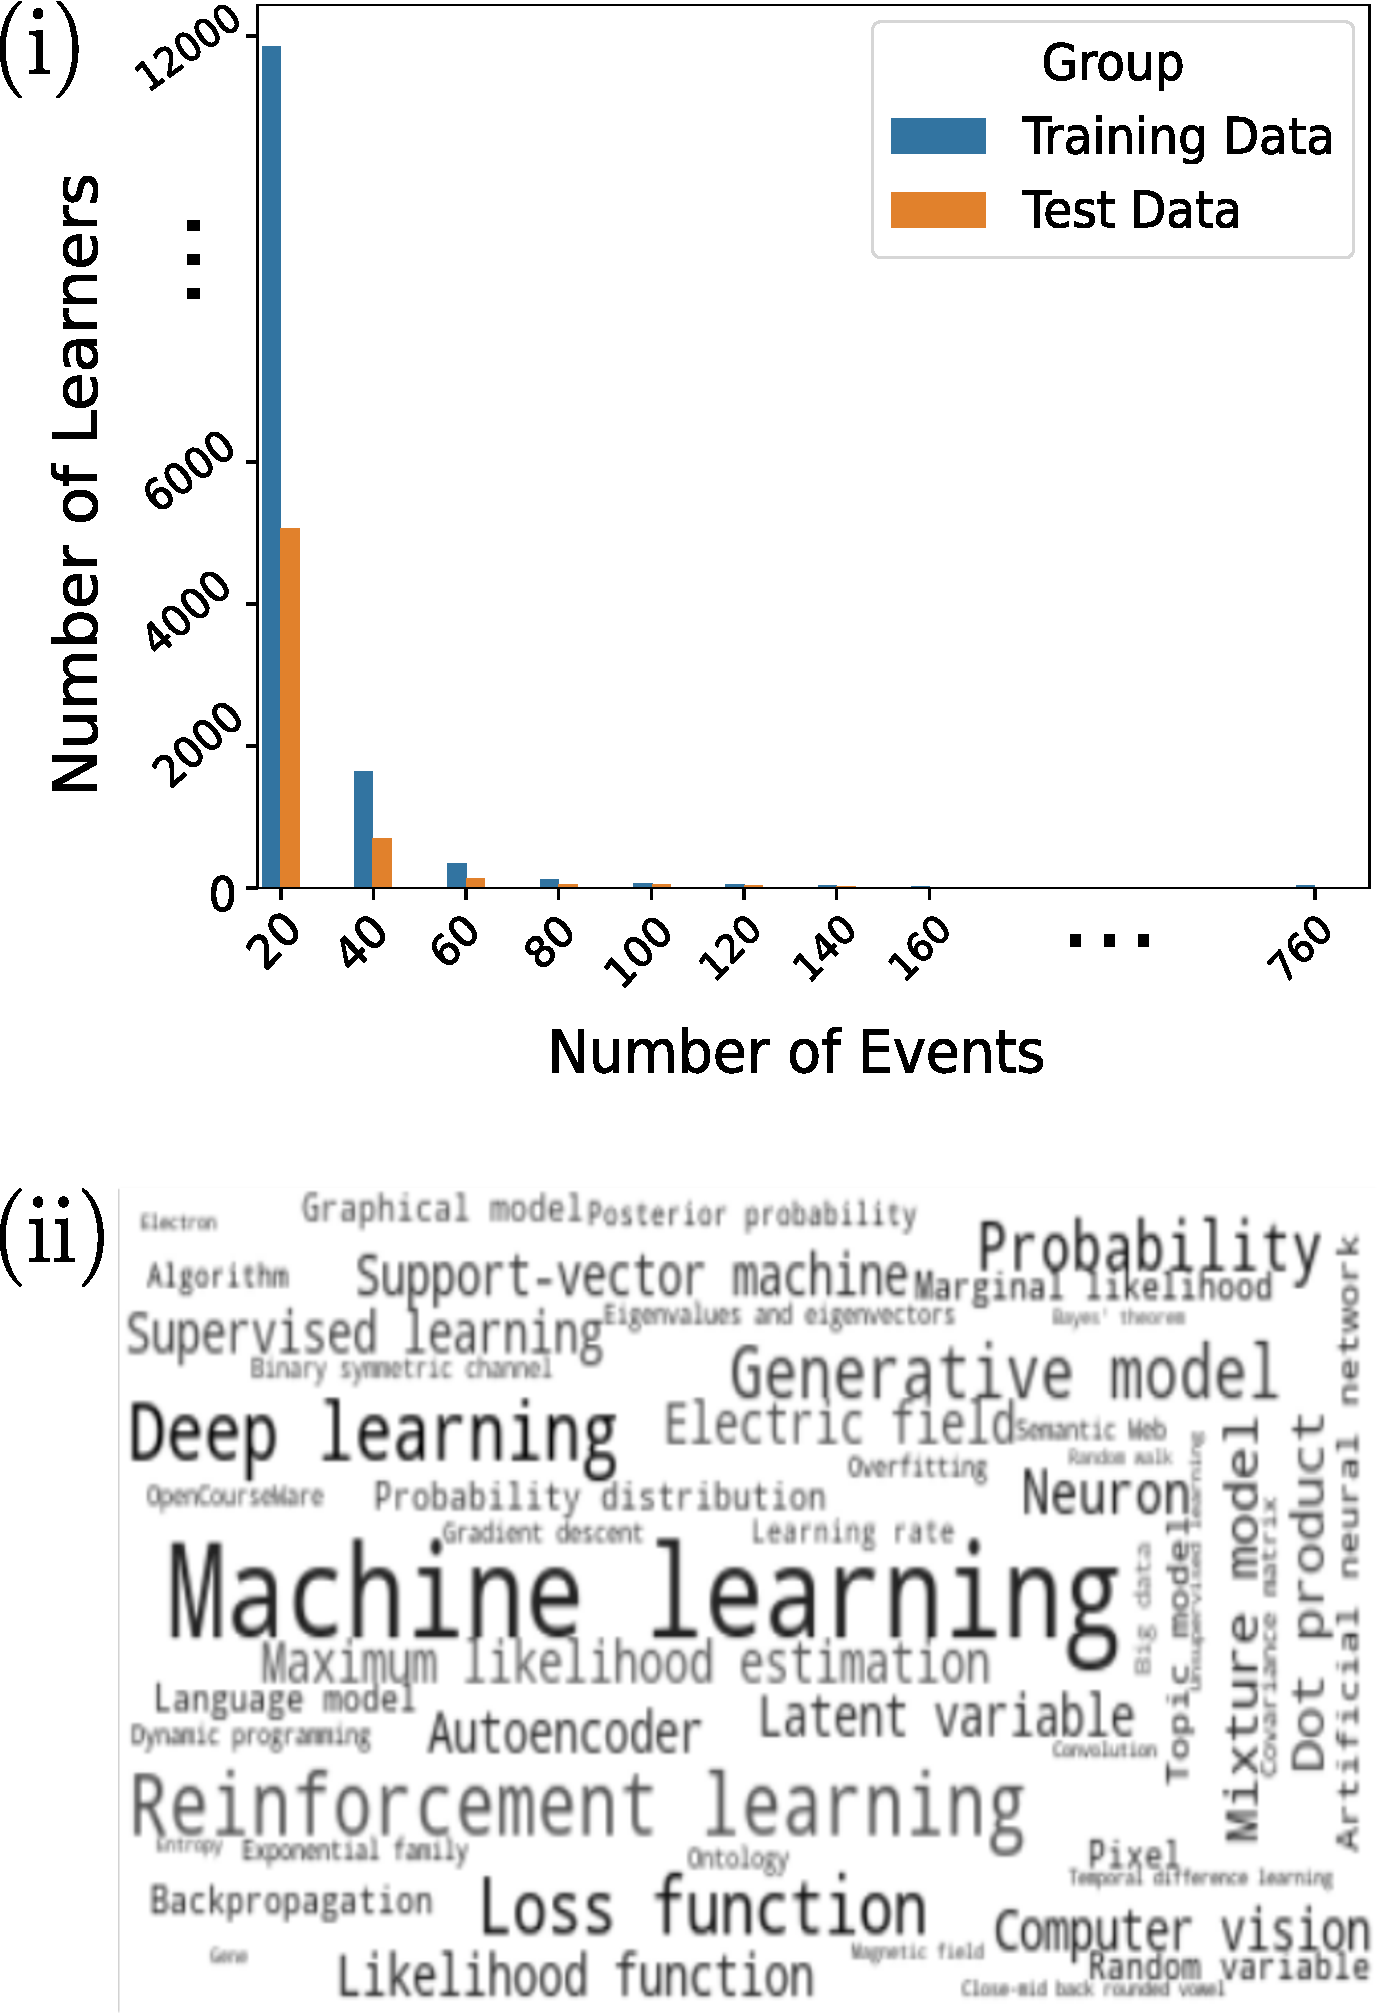
\includegraphics[width=.7\columnwidth]{dataset.pdf}}
    \caption{Characteristics of the PEEKC dataset: (i) number of learners in the training/test dataset based on the number of events in their sessions and (ii) wordcloud depicting the most frequent Wikipedia-based KCs showing the dominance of AI and ML concepts in the dataset.}
    \label{fig:dataset_stats}
\end{center}
\end{figure}



\begin{table}[] \small
\caption{Different columns included in the PEEKC Dataset.}
\label{tab:features}
\centering
\begin{tabular}{clc}
\hline
Column & Description & Data Type\\
\hline
1 & Video Lecture ID & Integer\\
2 & Video ID & Integer \\
3 & Part ID & Integer\\
4 & Timestamp & Integer \\
5 & User ID & Integer \\
6,8,10,12,14 & Knowledge Component IDs & Integer\\
7,9,11,13,15 & Topic Coverage & Floating Point\\
16 & Label & Binary\\
\hline
\end{tabular}
\end{table}


\section{\texttt{truelearn} Library}

This section describes the architecture of the TrueLearn Python library. While TrueLearn provides a probability that can be mapped to a binary outcome (engaging/not engaging), the probability prediction on different videos ranks them, creating personalised recommendations.



% According to Bayes rule the posterior distributions are proportional to:
% \begin{equation}
%  P(\theta^t_{\ell_{\texttt{I}}} | e^{t}_{\ell,r_x}, K_{r_x}, i_{r_x}) \propto P(e^{t}_{\ell,r_x} | \theta^t_{\ell_{\texttt{I}}}, K_{r_x}, i_{r_x}) \cdot P(\theta^t_{\ell_{\texttt{I}}})
% \end{equation}
% \begin{equation}
%  P(\theta^t_{\ell_{\texttt{NK}}} | e^{t}_{\ell,r_x}, K_{r_x}, d_{r_x}) \propto P( e^{t}_{\ell,r_x} | \theta^t_{\ell_{\texttt{NK}}}, K_{r_x}, d_{r_x}) \cdot P(\theta^t_{\ell_{\texttt{NK}}})
% \end{equation}


\subsection{Architecture}

The TrueLearn library consists of six modules.
% Figure \ref{fig:structure} outlines the main structure of the truelearn library.
% These modules are described below.

% \begin{figure}[ht]
% % \vskip 0.2in
% \begin{center}
% \centerline{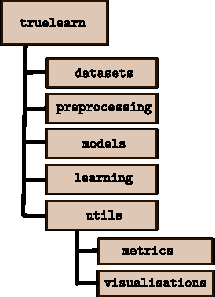
\includegraphics[width=0.5\columnwidth]{CameraReady/LaTeX/structure.pdf}}
% \caption{Library Structure of TrueLearn Library.}
% \label{fig:structure}
% \end{center}
% % \vskip -0.2in
% \end{figure}


% \subsection{Sub-packages}

\subsubsection{Datasets}
The dataset module integrates tools for downloading and parsing learner engagement datasets. Currently, the PEEKC dataset is integrated.
% New datasets can be integrated here to run experiments and use TrueLearn's learner-state visualizations.
% This module serves as a helper to integrate publicly available datasets that can be used for conducting experiments, evaluating model performance, and analysing learner data using TrueLearn’s visualisation capabilities.

\subsubsection{Pre-processing}
The pre-processing module contains utility classes for extracting content representations from educational materials. The extracted representations become KCs that can be used with IRT, KT and TrueLearn models. At present, utility functions for Wikification are included.

\subsubsection{Models}
This module houses the class that can store the learner model. In this context, the learner model refers to the data structure storing the learner state (e.g. knowledge/ interest). This learner model is loosely coupled with the learning algorithms which makes this object reusable with other learning algorithms that go beyond the TrueLearn algorithms.
% currently included in the library. This means that the output of other learning algorithms such as BKT and IRT can still be used to create learner representations using this class.
% In the models module, the term “models” refers to the structured representations of a learner, their knowledge, and learning events. These abstractions are used to organise and store learning-related data but should not be confused with machine learning models.

\subsubsection{Learning}
This module contains machine learning algorithms that can perform training and prediction of learner engagement with transcribed videos.
% Each classifier within this module follows an implicit interface inspired by scikit-learn design.
For training,  \texttt{fit} function is used. For prediction, \texttt{predict} and \texttt{predict\_proba} functions are used.
% to generate a binary label and a probability value respectively.
Currently, a set of baselines and the TrueLearn algorithms \cite{bulathwela2022sus} are included.

\subsubsection{Metrics}
Classification metrics accuracy, precision, recall and F1-score are built as the task is posed as a classification task in prior work \cite{truelearn}. The module is easily extendable to regression and ranking metrics.
% To evaluate the learning algorithm performance, the metrics module provides an interface to several key classification metrics including precision, accuracy, recall and F1 score. We use the scikit-learn API to support evaluation metrics. This opens up the opportunity to easily incorporate more evaluation metrics without having to put significant effort to test and maintain them in the future.

\subsubsection{Visualisations}
To effectively present the learner state, \emph{nine} different visualisations shown promising in prior work on user interaction \cite{mti6060042} have been developed.
% These visualisations can be used with the ability to sort the output based on specific study topics (KCs), based on learners’ proficiency.
\figurename{ \ref{fig:bubble}} provides a preview of one of the common visualisations. Seven (out of nine) interactive visualisations allow the learner to click and hover over the output to explore more details.
% \footnote{Examples: \url{https://truelearn.readthedocs.io/en/latest/examples/}}.
% However, they can also be saved as static images. The remaining two, namely, the Bubble Chart and Word Cloud, are exclusively static representations due to the limitations of the libraries used for their implementation.
% This module also provides the functionality to export these visualisations, where dynamic output can be saved in HTML format while the static output can be saved in various image formats such as png, jpeg and svg. This allows exporting the visual expressions to external systems (such as e-learning interfaces and printed materials).

\subsection{Visualising the Learner State}

% The visualisations that communicate the AI's learner state representation to a human user are implemented as part of the TrueLearn library.
Our approach was guided by a thorough examination of seminal research on impactful learning visualisations. Among others, the interactive visualisations designed in our Python library takes into account the goals of self-actualisation as detailed in the EDUSS framework \cite{mti6060042}.
% The visualisations in the TrueLearn library are inspired by the open learner model concept where models are developed to mainatain a humanly-intuitive representation \cite{bull2013visualising}
Additionally, the visualisations utilise user-friendly cues and conventions (colours/intensity of colour, shape size etc.) to minimise the cognitive load.
% Furthermore, the visualisations utilise user-friendly cues and conventions to minimise the learning curve for the human learner.
% Majority of visualisations present the \emph{current state} of the learner while there are also visualisations that can depict how the state of the learner evolves over time (where x-axis of the plot is time).
Based on user preferences found on learning visualisations \cite{visualisationscomparison}, the i) bar plot, ii) dot plot, iii) pie plot, vi) tree plot v) radar plot, vi) rose plot vii) bubble plot viii) word plot and ix) line plot were chosen to be implemented. Figure \ref{fig:bubble} previews the learner state of one of the learners.

TrueLearn algorithms model learner skill states as Gaussian variables with mean (state estimate) and variance (estimate uncertainty). The bar plot and dot plot use the bar/dot for skill mean while mapping the uncertainty as a confidence interval. The radar plot uses the radius of the radar as the skill estimate. The pie plot and tree plot use the area of the pie to represent skill mean while using the intensity of the colour (dark to light) for uncertainty. Rose plot, in addition to using the radius and colour intensity for mean and uncertainty respectively, uses the area of the pie to depict the number of video fragments that contributed to the skill estimate. The bubble plot and word plot use the size of the skill shape to represent the mean estimate, while the bubble plot uses the colour intensity to depict model uncertainty (\figurename{ \ref{fig:bubble}}). The line plot uses the x-axis as the time to show how a skill evolved over time. Popular learner models such as KT and IRT do not provide uncertainty for the skill estimate. Still, the implemented visualisations work without skill uncertainty values.
% The TrueLearn family of algorithms represents a state using a mean and a variance value. In two-dimensional plots such as bar plots and dot plots, the mean is the y-axis and the confidence intervals mark the variance. In circle-based plots such as bubble plots and rose plot, the radius of the circle represents the mean. The intensity of the colour maps to the variance of the estimate (dark being low variance).

% \begin{figure}[ht]
% % \vskip 0.2in
% \begin{center}
% \centerline{\includegraphics[width=.98\linewidth]{CameraReady/LaTeX/vis_plots.pdf}}
% \caption{A subset of the multiple visualisations available in the TrueLearn library to present the learner state in a humanly-intuitive way.}
% \label{fig:vis}
% \end{center}
% % \vskip -0.2in
% \end{figure}

% \section{Usage of truelearn Python Library}

% The truelearn Python library has two main uses, which are depicted in Figure \ref{fig:use}.

% \begin{figure*}[ht]
% % \vskip 0.2in
% \begin{center}
% \centerline{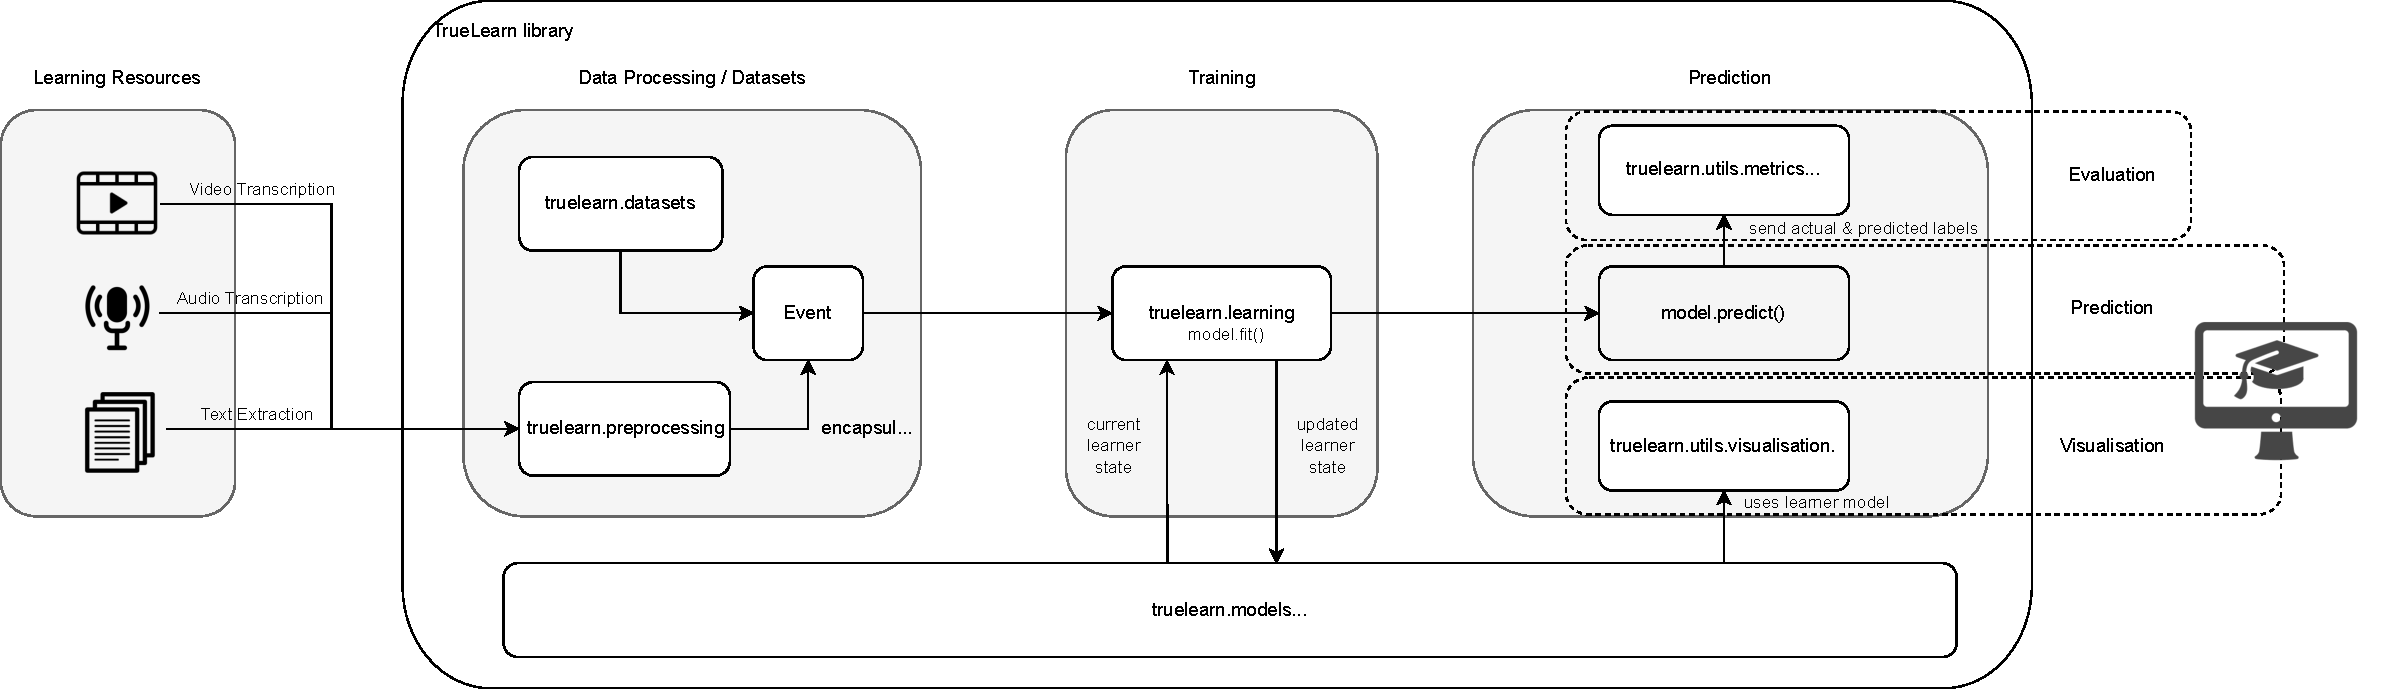
\includegraphics[width=\linewidth]{CameraReady/LaTeX/system.pdf }}
% \caption{Potential usage scenarios of the truelearn Python package to build an educational recommender within an e-learning system.}
% \label{fig:use}
% \end{center}
% % \vskip -0.2in
% \end{figure*}

% \subsection{Personalising E-learning/ Information}

% This Python package makes it very easy to incorporate personalisation into video-based e-learning platforms. The pre-processing module allows extracting KCs/topics from text transcriptions of video-based learning materials by associating them with Wikipedia topics. When a learner starts watching a video, the interaction signals can be recorded from the web application. The truelearn package can instantiate a learner model for each individual learner in the platform and use the interaction logs to update the learner model. The online learning algorithms can continuously fit the events to the learner model. The updated model can be used to predict engagement with a set of potential future videos (or any other type of educational material) to rank them and provide back to the learner as recommendations. Additionally, the learner may request to see their current state at any given point. The visualisation module can be used with the current learner state to create both static and interactive learner-state visualisations that can be presented to the end-user.

% \subsection{Offline/online Evaluation of Informational Recommenders}
% Academics and researchers can use the TrueLearn library for conducting both online and offline evaluation of educational/informational recommendation algorithms. If the researchers need to benchmark a new learning algorithm, they can implement the learner algorithm using the common interface provided by the TrueLearn library. Then the Python library can be integrated with a web application to run online experiments and record user interactions. Similarly, offline evaluations can be done either by using i) existing PEEKC dataset or ii) integrating a new dataset.




% \subsection{PEEKC Dataset}
% The dataset used for testing and evaluation was PEEKC, a Large Dataset of Learner Engagement with Educational resources \cite{PEEKC_orsum}. The dataset is structured in a way that provides information about the contents of each lecture and learners engagement with specific segments of it.

% Each lecture in the dataset has a unique identifier, with videos contained within it identified by their own ID. The videos are then divided into a series of fragments each with their own identifier that are associated with a maximum of 5 Knowledge Components that represent a specific topic or concept. The relevance of each Knowledge Component is determined using Cosine similarity, which measures the similarity between the content of the corresponding Wikipedia topic and the transcript of the video fragments.
% Learner IDs are used to identify individuals in the dataset, who are assigned a binary label to measure their engagement. A value of 1 indicates that they engaged with 75\% or more of the video segment, with 0 otherwise.

% Previously, the dataset mapped Knowledge Component IDs to their respective Wikipedia URL using an \texttt{url\_to\_id.csv} file. However, during the development of the TrueLearn library, this was improved to include both the title and description to provide a better understanding of each topic with this information embedded into the libraries Knowledge representation.

\section{Experiments and Results}

% Our objectives in running a rigorous prediction experiment with the proposed tools is two-fold.
We use the experimental protocol used in \cite{bulathwela2022sus} for our experiment.

\subsubsection{Baselines} We use a wide range of baselines that are i) exclusively content-based and ii) maintain a concept-based user model \cite{zarrinkalam2020extracting}. As content-based models, we use i) KC cosine similarity-based (\texttt{Cosine}), Jaccard similarity based on ii) KC intersection ($\texttt{Jaccard}_{\mathcal{C}}$) and iii) user intersection ($\texttt{Jaccard}_{\mathcal{U}}$). As concept-based user models, we use iv) TF (Binary), which counts the number of times a concept was encountered and v) TF (Cosine), which aggregates the cosine scores for skills in PEEKC dataset over time and vi) online Knowledge Tracing model (KT) \cite{bishopsnewbook}.

\subsubsection{TrueLearn Models} We use the three TrueLearn models implemented in the library, namely, i) TrueLearn Interest, capturing interests, ii) TrueLearn Novelty, capturing knowledge and novelty and iii) TrueLearn INK, combining interests, knowledge and novelty.

% \subsubsection{Dataset} We use the proposed PEEKC dataset.

\subsubsection{Data and Evaluation} For each learner, its engagement at time $t$ is predicted using its events at times $1$ to $t-1$. We used the hold-out validation (70\% train/ 30\% test) technique in our experiment where the training data in PEEKC is used for hyperparameter tuning of models. The best hyperparameter combination based on the F1-Score is identified and used with the test set to evaluate the reported performance. Since the engagement is labelled as a binary label in the PEEKC dataset, accuracy, precision, recall, and F1 score are reported.
% In order to validate the accuracy of the implementation, we ran a few small-scale experiments attempting to replicate the results published in prior work \cite{bulathwela2022sus}. We used the PEEKC dataset \cite{PEEKC_orsum} to evaluate the performance of the primary TrueLearn models proposed in prior work, namely, i) TrueLearn Interest and TrueLearn Novelty. The experimental protocol was similar to the one used earlier.
% % We conducted a series of experiments using the PEEKC dataset presented above to verify that the library was able to replicate the results obtained in the previous truelearn paper.
% We also used a sequential experimental design. For each learner, its engagement at time $t$ is predicted using its engagement at times $1$ to $t-1$. We used the hold-out validation technique in our experiments where the training data is used for hyperparameter tuning. The best hyperparameter combination based on the F1-Score is identified. This combination is used with the test set to evaluate the final predictive performance. Since the engagement is predicted as a binary label in the PEEKC dataset, the predictions for each event can be combined into a confusion matrix to compute accuracy, precision, recall, and F1 score. Same as in the prior publications, we calculate the weighted average of each learner's metrics based on their number of events.

% Q: How to reference the hyperparameters we used?
% \textbf{Hyperparameters}: For initial hyperparameters, we initialised the initial mean skill of learners to 0 for all models and use grid search to find the suitable hyperparameters for the initial variance and beta value.

\subsection{Empirical Evaluation}

The results are reported in Table \ref{tab:results}. Our experiments i) guarantee the correctness of the library implementation and ii) demonstrate the predictive capabilities of the web-scale online learning models with comparable baselines.

% Q: How to properly reference previous results?
% \textbf{TrueLearn Novelty vs. TrueLearn Knowledge:} The experimental results show that TrueLearn Knowledge has the highest Acc. value, which validates the results in previous truelearn paper. In terms of recall and F1, TrueLearn Novelty outperforms TrueLearn Knowledge, which proves the need to exploit learner novelty and demonstrates that TrueLearn Novelty is indeed more competitive compared to TrueLearn Knowledge.

% \textbf{TrueLearn Interest vs. TrueLearn Novelty:} TrueLearn Novelty showed higher performance than TrueLearn Interest, as expected. Specifically, TrueLearn Novelty exhibited better performance than TrueLearn Interest in Acc., Prec., Rec. and F1.

% \section{Emperical Results}

\begin{table}[] \small
\caption{Performance of TrueLearn algorithms are evaluated using Precision (Prec.), Recall (Rec.) and F1 Score (F1). The best and second best performance is indicated in \textbf{bold} and \emph{italic} faces respectively. TrueLearn models outperform the best baseline most times ($p< 0.01$ in a one-tailed paired t-test are marked with $\cdot^{*}$).}
\label{tab:results}
\begin{tabular}{cccccc}
\hline
& Model              & Acc. & Prec. & Rec. & F1    \\
\hline
% \texttt Persistence  & \textit{55.08} & \textit{57.86} & 58.45 & 54.06 \\
% \texttt Majority & \textit{73.635} & \textit{57.859} & 58.451 & 54.056 \\
&\texttt{Cosine}& {55.08} & {57.86} & 58.45 & 54.06 \\
&$\texttt{Jaccard}_{\mathcal{C}}$& 55.46 & 57.81 & 60.36 & 55.03 \\
Baselines&$\texttt{Jaccard}_{\mathcal{U}}$ & 64.06 & 57.85 & {72.76} & {61.22} \\
&TF (Binary)	& 55.19 &	56.71 & 66.60 &	57.38 \\
&TF (Cosine) & 55.11 &	56.75	& 65.95	 & 57.11 \\
&KT & 54.99 & 53.25 & 28.56 & 34.51 \\
\hline
&Interest & 58.13    & 52.08     & \textit{78.61}$^{*}$  & 63.00$^{*}$ \\
% TrueLearn Novelty  & 65.65	  & 59.23	  & 79.81  & 65.71 \\
TrueLearn & Novelty  & \textit{64.78}$^{*}$	  & \textit{58.52}$^{*}$  & \textbf{80.91}$^{*}$  & \textbf{65.53}$^{*}$ \\
&INK  & \textbf{78.32}$^{*}$	  & \textbf{64.32}$^{*}$	  & {64.03}  & \textit{64.00}$^{*}$ \\
\hline
\end{tabular}
\end{table}



%\textbf{Example}: The bubble chart visualisation is valuable for students to gauge their proficiency across multiple subjects. In the example below, the bubble chart visualises the mean and variance across the learner's top 15 subjects. The dimensions of the bubbles represent the mean values, while the intensity of the green colouring corresponds to the variance. As indicated by the provided legend, a darker shade of green signifies greater confidence in our algorithm's prediction, thus indicating a lower variance.


\begin{figure}[]
% \vskip 0.2in
\begin{center}
\centerline{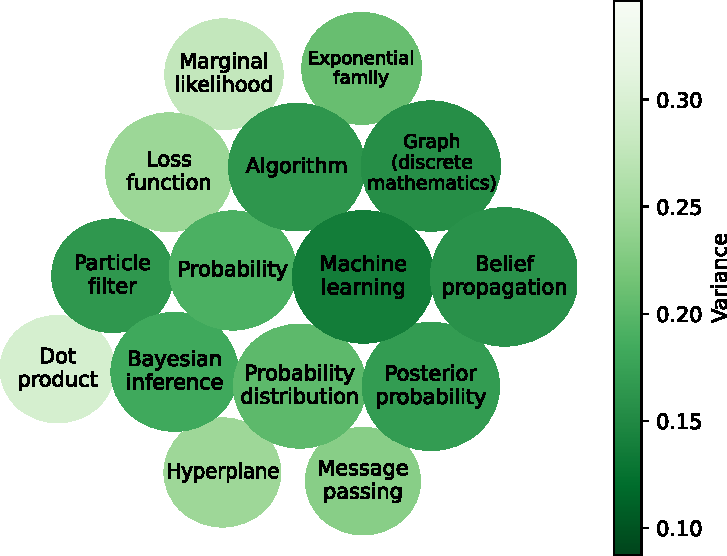
\includegraphics[width=.7\linewidth]{visual_plot.pdf}}
 \caption{The 15 most knowledge acquired KCs of a learner in a bubble plot. The size of the circle aligns with the KC mean and the intensity of the colour maps to the variance.}
\label{fig:bubble}
\end{center}

% \vskip -0.2in
\end{figure}

% \begin{figure}[]
% % \vskip 0.2in
% \begin{center}
% \centerline{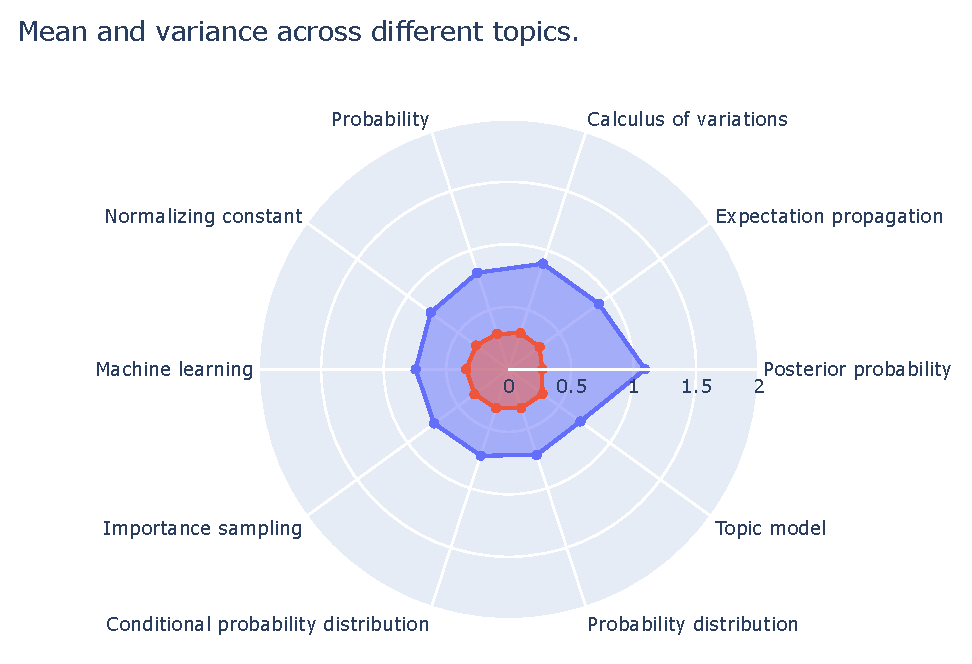
\includegraphics[width=0.95\columnwidth]{icml2023/radar_chart.pdf}}
% \caption{}
% \label{fig:radar}
% \end{center}
% % \vskip -0.2in
% \end{figure}


\section{Discussion}

The contributions in this work span over a novel dataset, an OLM library and empirical experiments.

\subsection{PEEKC for AI Education}
As per the wordcloud in \figurename{ \ref{fig:dataset_stats} (ii)}, the videos in the PEEKC dataset are swamped with AI and ML-related KCs. PEEKC's data source, VLN repository extensively visits AI conferences which causes this effect. But, this makes PEEKC a perfect dataset to understand in-the-wild video-based knowledge acquisition, making this dataset an excellent resource for training personalisation models for AI education as we have done in table \ref{tab:results}. While we haven't demonstrated here, the dataset is potentially valuable for unsupervised tasks such as pre-requisite identification and hierarchical structuring of concepts in AI. A key benefit of PEEKC dataset is the ability to use the methodology in \figurename{ \ref{fig:peek_pipe}} with VLN repository to create larger datasets in the future.


\subsection{TrueLearn Performance and Visualisations}
% We designed visualisations, to empower students to recognise, contrast, and track the development of their skill level across subjects of their choice. It employs our algorithms’ prediction of their skill level (‘mean’) and calculation of a certain level in these predictions (‘variance’). These computations stem from learners' interaction with diverse learning resources and subject matters, classified based on Wikipedia topics.

Table \ref{tab:results} clearly shows the superiority of the TrueLearn model implementations in comparison to the comparative baselines aligning with prior work's evidence \cite{bulathwela2022sus}. The most expensive, \verb|fit| function measures $0.005\pm0.0036s$ to execute in an Apple M1 3.2GHz CPU. TrueLearn states of each learner in the dataset can be constructed in parallel because there are no inter-learner dependencies, also making the model privacy-preserving by design. The performance in table \ref{tab:results} coupled with event counts in \figurename{ \ref{fig:dataset_stats}} shows the data efficiency of TrueLearn, which is able to learn from a very small number of events.

The library is designed to enable learners to effortlessly generate dynamic and static visualisations, promoting a learner-centric, self-regulated study experience \cite{bull2008metacognition}. \figurename{ \ref{fig:bubble}} previews the learner knowledge state from one of the learners in the PEEKC test data. It is seen that the visualisation demonstrates how the user is acquiring knowledge in AI-related topics, specifically, in the area of Bayesian modelling.
% Even if the user is not aware of a KC shown in the visualisation, they can easily go to Wikipedia to learn the definition.
The EDUSS framework-inspired visualisations support development by translating skill-level predictions into visual progress indicators encouraging continuous learning. Understanding is enhanced by providing insights into learners' interaction patterns, promoting self-awareness \cite{mti6060042}. The transparency of the user model allows learners to scrutinise their learning progress and engage critically with the underlying data (while ways to provide this feedback to the model is still an open research area). Finally, by making the visualizations shareable, the library fosters social interaction, adding a community dimension to the learning experience and improving its usability to other stakeholders of education (e.g. parents and teachers).
% In short, through the effective amalgamation of seminal research with innovative programming, our library empowers learners to be active participants in their educational journey, embodying the principles of self-actualization.


% properly cite these two papers
% Our approach was guided by a thorough examination of seminal research on impactful learning visualisations. Among others, the visualisations designed in our Python library take into account the goals of self-actualisation as detailed in the EDUSS framework. Our visualisations aim to facilitate not just learning but also personal growth, following the tenets of the framework. Each aspect of the EDUSS framework has been carefully considered in the development of these visualisations. These visualizations inspire exploration, by presenting various learning resources in an engaging, interactive format. They also support development, translating skill level predictions into visual progress indicators to encourage continuous learning. Understanding is enhanced by providing insights into learners' interaction patterns, promoting self-awareness. The transparency of the user model used allows learners to scrutinize their learning progress and engage critically with the underlying data. Finally, by making the visualizations shareable, the library fosters social interaction, adding a community dimension to the learning experience. In short, through the effective amalgamation of seminal research with innovative programming, our library empowers learners to be active participants in their educational journey, embodying the principles of self-actualization.

% By incorporating the results from the questionnaire responses \cite{visualisationscomparison}, we arrived at a selection of nine distinct visualisation types: Bar Charts, Line Charts, Dot Plots, Pie Charts, Rose Charts, Bubble Charts, Tree Maps, Radar Charts, and Word Clouds.

\subsection{Library Design, Stability and Maintainability}

The adherence to prior work-inspired good practices and API design makes using the TrueLearn library developer-friendly for both offline experimentation and e-learning system integration. Using a collection of base classes that define a common interface and shared functionality similar to scikit-learn-like estimators with \verb|fit| and \verb|predict| functions \cite{buitinck2013api} reduces the learning curve while the design allows elaborate type and value checks when the hyperparameters of the classifiers are modified, ensuring the robustness of the classifier implementation.
% This pattern establishes a foundation that can be easily extended and customised moving forward.
The decoupling of the feature-engineering from modelling modules allows users to extend the capability of the library with new KC extraction functions (beyond Wikification), new online learner models and open learner visualisations without having to worry about interdependencies. Detailed instructions are provided to developers with style guides and design principals \footnote{Contributing: \url{https://truelearn.readthedocs.io/en/latest/dev/}} to ease contribution. The core research team is committed to maintaining the library in the future while providing further guidance and code reviews when extending the capabilities of the library.
% Throughout the development process, we adhere to design principles discussed in related work, such as consistency, inspection, and hybrid types. By providing a consistent training and prediction interface for all classifiers in the truelearn library, we have achieved the consistency principle. Simultaneously, for easy inspection, we exposed the internal state of objects by means of property attributes, public attributes, and getters/setters. The reason why we use getters/setters instead of public attributes in the classifier is to better facilitate the hybrid typing approach. With these methods, we can perform type and value checks when the hyperparameters of the classifier are modified, which ensures the robustness of the classifier implementation and guides the user to pass in the correct hyperparameters. Considering that users may want to implement their version of the KC (in order to include custom topic fields needed by their subject domain), truelearn classifier interacts with the KC by using static duck typing whenever possible, which promotes interoperability between truelearn and client code as well as the scalability of truelearn itself.
% \subsection{Stability}
Furthermore, TrueLearn benefits from 100\% test coverage achieved through a combination of integration, unit, and documentation tests.
% These tests were run on python versions ranging from 3.7 to 3.11 on all major operating systems to ensure compatibility. By making use of periodic testing with Continuous Integration, we can more greatly ensure that TrueLearn will work as intended regardless of the operating environment.

% \subsection{Maintainability}

% Modularity is an important aspect of the TrueLearn library, achieved by using a collection of Base classes that define a common interface and shared functionality . This design allows establishes a foundation that can be easily extended and customised moving forward.
% To ensure the straightforward integration of the TrueLearn library, our documentation includes a wide range of examples showcasing the functionality offered by our API and visualisations. These examples are accompanied by the necessary code to generate them, allowing for a clear understanding of their implementation.
% To further enhance maintainability, we have taken several additional measures. Firstly, we focused on minimising external dependencies wherever feasible to reduce the risk of compatibility issues and make it easier to maintain our codebase independently.
Code consistency and readability are further enhanced by following the PEP 8 guidelines \cite{pep8}, which define a set of best practices for Python code. Extensive documentation
% \footnote{Documentation at \url{https://truelearn.readthedocs.io/en/latest/}}
of the modules and classes with in-context code examples describes relevant information for both a potential developer and a contributor to familiarise themselves with the library. Developers have already started adapting this library to learning platforms \cite{x5learn}. We aim to objectively assess their experience by surveying them \cite{piccioni2013empirical,nadi2023selecting}.

% Furthermore, we provide a comprehensive API reference, offering detailed information for each class and function. The project website \footnote{Available at \url{https://truelearn.readthedocs.io/en/latest/}} describes relevant information for both a potential end-user or a contributor to familiarise with the library. Each of these comes with its own fine-grained examples along with descriptions of their purpose. To better explain the rationale of the technical and design decisions made, information is provided concerning the library's design and style guide in the \emph{contributing} section to minimise the learning curve associated with future development.
% The project website extensively describes the



\subsection{Relevance, Impact and Limitations}

{Modelling learner state in a humanly intuitive manner, requiring minimal data and exclusively relying on individual user actions, TrueLearn offers a transparent learner model that respects the privacy of its users and can scale to lifelong education. The development of the TrueLearn library aims to provide both the research and developer communities with the opportunity to seamlessly use the TrueLearn family of models in their work. The learner models utilise Wikipedia-based entity linking to create KCs based on a publicly available knowledge base. The content annotation can also scale to thousands of materials created in different modalities (video, text, audio etc.).}

{The impact of TrueLearn is two-fold. For developers and researchers, the TrueLearn library employs a design that conforms with popular machine learning libraries. The documentation is extensive and contains detailed examples that help the implementation. For developers and educators, probabilistic graphical models that are data efficient and humanly intuitive are available to be used in their downstream systems. The engagement predictions (between values 0 and 1) can be used to rank videos for personalised learning. Combined with the PEEKC dataset, hyperparameters for a new system can be trained beforehand and deployed in a new online learning platform. The online learning algorithm updates the learner state in real-time helping better personalisation. A platform implementing TrueLearn can scale to a large population of users and support them through lifelong education due to the large number of KCs it can support.}

% In an era where AI is reaching a position that can impact society significantly, TrueLearn library unlocks the power of personalisation of information while taking into account multiple human values that go beyond knowledge management (e.g. climate responsibility, privacy, transparency to name a few).

% \subsection{Limitations}

{While getting inspired by scikit-learn library, the learning algorithms in TrueLearn library are not compatible with some helper functions available in scikit-learn (such as grid search) and pandas libraries at this point. Building seamless compatibility with these utilities will enable the TrueLearn library to be adopted by a wider audience while minimising the development effort required to support such powerful features. While the visualisations implemented are time-tested \cite{visualisationscomparison,mti6060042}, their success with TrueLearn representations has room for rigorous understanding via user studies. The exclusive support of online learning algorithms can also be seen as a limitation of the current library as many batch learning algorithms are proposed for educational recommendation and engagement modelling \cite{intervention_bkt,ensemble_kt}. While learner engagement is a prerequisite for learning, it is noteworthy that learner engagement doesn't imply learning. The library also does not support state-of-the-art deep learning algorithms \cite{deep_kt,pardos_serendipity} that may be useful where interpretability and learner state visualisation are not the top priority.}

%Further to open learner modelling, TrueLearn employs Wikipedia, helping the democratisation of education \cite{democratise2021}. %The data and computational efficiency of the models also lead to minimised carbon footprint.
%The models are currently used in building a platform that connects Open Educational Resources to lifelong learners supporting lifelong, equitable education.

% Karim: I wonder if this is better placed in Limitations?
% \textbf{Interoperability between truelearn and scikit-learn:} Currently, truelearn's classifier does not interoperate well with scikit-learn (e.g., using scikit-learn's grid search to find the right hyperparameter). The main problem comes from scikit-learn's requirement for the parameters of the `fit` function, which demands that the data for training the model (parameter X) be an array of shape \texttt{(n\_samples, n\_features)} where \texttt{n\_samples} denotes the number of samples and \texttt{n\_features} denotes the number of features. However, in the truelearn classifier, \texttt{fit} only takes in a single learning event. This makes it necessary for users to maintain a separate grid search algorithm when using truelearn, which increases the maintenance burden and the difficulty of reusing the code.


\section{Conclusion}
% \section{Summary of the System}

{This work presents \textit{PEEKC} dataset and \textit{TrueLearn} Python library, creating a valuable toolbox for engagement modelling with AI-related educational videos. The library contains several online learning models, which model multiple factors influencing learner engagement. It also packages a set of visualisations that can be used to interpret the learner's interest/knowledge state. The learner representations and state visualisations are comparable to outputs of knowledge tracing models, except TrueLearn uses watch time interactions rather than relying on test taking. The empirical results demonstrate that the implementation of the library achieves similar performance to the prior work. The new implementation encourages educational data mining practitioners to use this library to incorporate educational video recommendations in e-learning systems. Researchers are encouraged to extend this library with new datasets and online learning algorithms for learner engagement modelling.}

% \subsection{Future Work}
The immediate future work entails improving learner state visualisations via user studies.
% running several user studies to evaluate the effectiveness of the visualisations and identifying ways to improve them.
Integrating the library into a real-world e-learning platform \cite{10.1145/3397482.3450721} is a top priority.
% Incorporating the library into a real-world e-learning platform to run online evaluations is also a top priority.
Extending the current framework to podcasts and other information content while incorporating other feedback forms like educational questions \cite{bulathwela2023scalable,bulath2023neurips} remains in the future roadmap.
% We also aim to evaluate the performance of the TrueLearn models in the context of information recommenders that present informational content such as news and podcasts to demonstrate the generalisability of the models. Incorporating models that can exploit explicit feedback simultaneous to implicit feedback can also enhance the library and its utility.
In the long term, we aim to add more general informational recommendation algorithms to the library and mobilise the research community to contribute various models, pre-processing techniques and evaluation metrics that the library can benefit from.

\section{Acknowledgments}
This work is partially supported by the European Commission-funded project "Humane AI: Toward AI Systems That Augment and Empower Humans by Understanding Us, our Society and the World Around Us" (grant 820437) and the X5GON project funded from the EU's Horizon 2020 research programme grant No 761758.

\clearpage
\bibliography{aaai24}
% Guesmi, M.; Chatti, M.A.; Tayyar, A.; Ain, Q.U.; Joarder, S. Interactive Visualizations of Transparent User Models for Self-Actualization: A Human-Centered Design Approach. Multimodal Technol. Interact. 2022, 6, 42. https://doi.org/10.3390/mti6060042


% \begin{table*}[]
% \caption{Detailed descriptions of the different columns of the \texttt{train.csv} and \texttt{test.csv} files included in the PEEKC Dataset.}
% \label{tab:features}
% \centering
% \begin{tabular}{ccl}
% \hline
% Column & Description & Details \\
% \hline
% 1 & Video Lecture ID & An integer ID associated with an individual video lecture \\
% 2 & Video ID & An integer ID associated to every video belonging to the same Video Lecture ID (e.g. $1\dots v$ \\
% & & if the lecture has $v$ videos) \\
% 3 & Part ID & An integer ID associated with each video fragment (e.g $1 \dots f$ for a video with $f$ fragments) \\
% 4 & Timestamp & Timestamp (to the nearest second) when the play event was initiated. \\
% 5 & user ID & An integer ID associated with each unique learner in the dataset PEEKC dataset (IDs in \\
% & & \texttt{train.csv} and \texttt{test.csv} files are mutually exclusive). \\
% 6,8,10,12,14 & KC IDs & An integer ID associated with each unique Knowledge Component. This ID can be linked to  \\
% & & the human readable Wikipedia concept names found in \texttt{id\_to\_wiki\_url\_mapping.csv} file \\
% 7,9,11,13,15 & Topic Coverage & Proxy for coverage of the relevant KC in the fragment of interest. KC   coverage is the cosine \\
% & & similarity as per equation \ref{eq:wiki_cos}. \\
% 16 & Label & The binary label $e^t_{\ell,r_i}$, 1 if the learner watched $\geq$ .75 of the video  fragment, 0 otherwise.\\
% \hline
% \end{tabular}
% \end{table*}

% \newpage
\section{Supplementary Material}

\subsection{Detailed Problem Setting}

A learner $\ell$ in learner population $L$ interacting with a series of educational resources $S_\ell \subset \{r_1, \ldots, r_{R}\}$ where $r_x$ are \emph{fragments/parts} of an educaitonal video $v$. The watch interactions happen over a period of $T$ time steps, $R$ being the total number of resources in the system.
In this system with a total $N$ unique knowledge components (KCs), resource $r_x$ is characterised by a set of top KCs or topics $K_{r_x} \subset \{1, \ldots, N \}$. We assume the presence $i_{r_x}$ of KC in resource $r_x$ and the degree $d_{r_x}$ of KC coverage in the resource is observable.

% TODO: {-1, 1} or {0, 1}?
The key idea is to model the probability of engagement $e_{\ell, r_x}^{t} \in \{ 1, -1\}$ between learner $\ell$ and resource $r_x$ at time $t$ as a function of the learner interest $\theta^t_{\ell_{\texttt{I}}}$, knowledge $\theta^t_{\ell_{\texttt{NK}}}$ based on the top KCs covered $K_{r_x}$ using their presence $i_{r_x}$, and depth of topic coverage $d_{r_x}$.

\begin{figure}[H]
\begin{center}
\centerline{\includegraphics[width=0.65\columnwidth]{problem_setting.pdf}}
\caption{Visual illustration of the problem setting where learner $\ell$, with knowledge (that allows them to tackle novel content) $\theta_\texttt{NK}$ and interests $\theta_\texttt{I}$ is watching fragments of educational videos $r_x$ containing different knowledge components $K_{r_x}$ over time $t$.}
\label{fig:semantic_rel_problem}
\end{center}
% \vskip -0.2in
\end{figure}

\subsection{Baseline Models}
% \subsection{Baseline Models}

PEEKC is the first of its kind, a dataset that records in-the-wild  engagement of informal learners with video lecture fragments. Due to the novelty of this dataset, we struggle to find already published baselines, except for the TrueLearn family of algorithms.
For the sake of comparing its predictive performance,  we also propose a set of baselines that are based on content-based and collaborative filtering.

\paragraph{Content-based Similarity} Content-based filtering can measure the similarity between two items. We compute a similarity value, $sim(r^{t-1}_{\ell,r_i},r^{t}_{\ell,r_i})$ between two consecutive lecture fragments $r^{t-1}_{\ell,r_i}$ and $r^{t}_{\ell,r_i}$ in the learner  $\ell$'s session. We use this similarity value to make an engagement prediction $\hat{e}^t_{\ell,r_i}$ based on equation \ref{eq:cbf_baseline}.

\begin{equation} \label{eq:cbf_baseline}\centering
    \hat{e}^t_{\ell,r_i} =
    \left\{
      \begin{array}{ c l }
        1                 &  if\ sim(r^{t-1}_{\ell,r_i},r^{t}_{\ell,r_i}) \geq threshold \\
        0                 & otherwise
      \end{array}
    \right.
\end{equation}

In this case, we investigate two similarity measures, namely 1) \emph{Cosine}, 2) \emph{Concept-based Jaccard} and \emph{User-based Jaccard}. When computing cosine similarity, we represent each video fragment using the bag of concepts representation where the concepts are the superset of Wikipedia concepts mentioned in the dataset. The values in this sparse vector are the cosine similarities between the respective Wikipedia concept and the lecture fragment transcript as per equation \ref{eq:wiki_cos}.

\begin{equation}\label{eq:wiki_cos}
        cos(s_{tr}, c) = \frac{\texttt{TFIDF}(s_{tr}) \cdot \texttt{TFIDF}(c)}
        {\|\texttt{TFIDF}(s_{tr})\| \times \|\texttt{TFIDF}(c)\|}
\end{equation}

An alternative approach to finding concept-wise similarity is Jaccard similarity. Concept-based Jaccard similarity $\texttt{Jaccard}_{\mathcal{C}}(r^{t-1}_{\ell,r_i}, r^{t}_{\ell,r_i})$,  between lecture fragments $r^{t-1}_{\ell,r_i}$ and $r^{t}_{\ell,r_i}$ is computed based on equation \ref{eq:concept_jaccard}.

\begin{equation} \label{eq:concept_jaccard}\centering
    \texttt{Jaccard}_{\mathcal{C}}(r^{t-1}_{\ell,r_i}, r^{t}_{\ell,r_i}) =
    \frac{\mathcal{C}(r^{t-1}_{\ell,r_i}) \cap \mathcal{C}(r^{t}_{\ell,r_i})}
    {\mathcal{C}(r^{t-1}_{\ell,r_i}) \cup \mathcal{C}(r^{t}_{\ell,r_i})}
\end{equation}
where $\mathcal{C}(\cdot)$ is a function that returns the set of Wikipedia concepts in resource $r_i$

Similarly, one can also measure the similarity between two lecture fragments based on how many learners interact with both lecture fragments. The user interactions in the training dataset is used exclusively to learn the similarity matrix in order to avoid data leakage. In this approach, we can calculate the user-wise Jaccard similarity $\texttt{Jaccard}_\mathcal{U}(r^{t-1}_{\ell,r_i}, r^{t}_{\ell,r_i})$, as per equation \ref{eq:user_jaccard}.

\begin{equation} \label{eq:user_jaccard}\centering
    \texttt{Jaccard}_\mathcal{U}(r^{t-1}_{\ell,r_i}, r^{t}_{\ell,r_i}) =
    \frac{\mathcal{U}(r^{t-1}_{\ell,r_i}) \cap \mathcal{U}(r^{t}_{\ell,r_i})}
    {\mathcal{U}(r^{t-1}_{\ell,r_i}) \cup \mathcal{U}(r^{t}_{\ell,r_i})}
\end{equation}
where $\mathcal{U}(\cdot)$ is a function that returns the set of learners that interacted with resource $r_i$

\paragraph{Knowledge Tracing (KT)}

KT builds a learner representation of the knowledge of the learner. This learning model is then used in predicting the engagement of learner $\ell$ with lecture fragment resource $r_i$ at time $t$. As the PEEKC dataset has a temporal dimension, we reformulate the KT algorithm into an online learning graphical model inspired by the reformulation found in prior work.  The skill variables in the KT model are Bernoulli variables ($\theta^t_{\ell,c} \sim \texttt{Bernoulli}(\pi^t_{\ell,c})$), assuming that a learner $\ell$ would have either mastered a skill/ concept $c$ or not (represented by probability $\pi^t_{\ell,c}$). Skills are initialised ($\theta^0_{\ell,c}$) using a $\texttt{Bernoulli}(.0)$ prior, assuming that the latent skill is not mastered in the beginning. A noise factor similar to what is found in the conventional KT model is added to this model and is tuned using a grid search.

% \newpage
\subsection{Number of Knowledge Components Published with the PEEKC Dataset}

\begin{figure}[h]
%\vskip 0.2in
\begin{center}
    \centerline{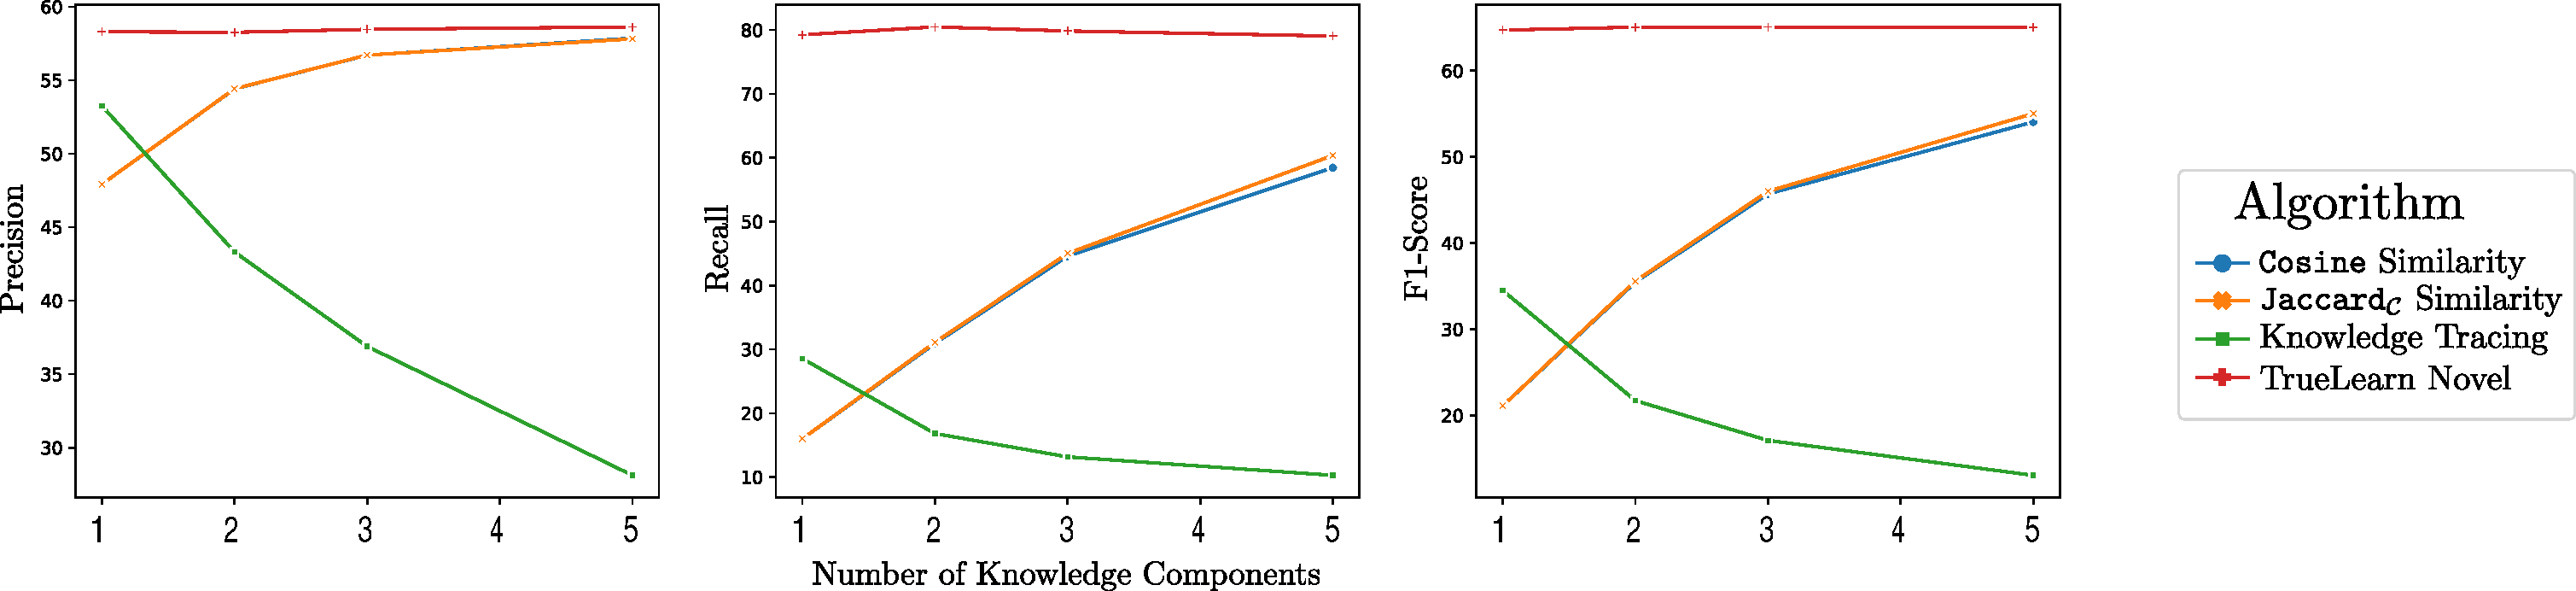
\includegraphics[width=1.1\linewidth]{results_plot.pdf}}
    \caption{Predictive performance on PEEKC dataset test data in terms of Precision (left), Recall (middle) and F1-Score (right) for the benchmark models when varying numbers of Knowledge Components (KCs) are used as the content representation. Higher number of topics did not increase the performance of the Cosine and Jaccard models significantly to reach TrueLearn Novelty model}
\end{center}
%\vskip -0.2in
\end{figure}

\subsection{Hyperparameters for Reproducing Experiments}

\begin{table}[h] \footnotesize
\caption{The hyperparameter combinations that produced the results that are reported in the results section.}
\centering
\begin{tabular}{c c l c}
  \hline
    Sec. &  Model & Relevant Hyperparameter & Value \\
  \hline
  1 & & Draw Probability & 0.52\\
  & TrueLearn& Initial Variance & 300.00 \\
  & Interest& Beta & 8.83 \\
  & & Tau & 0.0\\
  & & Best Hyperparameter Set & Max. F1-Score \\
  \hline
 2 & & Draw Probability & 0.52\\
  & TrueLearn& Initial Variance & 0.25 \\
  & Novelty& Beta & 0.42 \\
  & & Tau & 0.0\\
  & & Best Hyperparameter Set & Max. F1-Score \\
  \hline
  3 & & Greedy & True\\
  & & Tau & 0.5\\
  & TrueLearn & Interest Model & Model in Sec. 1 \\
  & INK & Novelty Model & Model in Sec. 2 \\
  & & Best Hyperparameter Set & Max. F1-Score \\
   \hline
\end{tabular}
\end{table}

\subsection{Computational Complexity}

The execution time benchmarks were carried out using a laptop computer with an Apple M1 3.2GHz CPU and 16GB RAM.

\begin{table}[h!] \footnotesize
\caption{The mean duration with the standard error (1.96 $\times$ standard deviation) taken for a function execution of a single event of a single learner in the PEEKC dataset.}
\centering
\begin{tabular}{l c c}
  \hline
  Function & TrueLearn Model & Execution Time (s) \\
  \hline
  & Interest & 0.002016 $\pm$ 0.00478
  \\
  \texttt{fit()} & Novelty & 0.002232 $\pm$ 0.00468 \\
   & INK & 0.005000 $\pm$ 0.00712 \\
   \hline
  & Interest & 0.000084 $\pm$ 0.000020   \\
  \texttt{predict\_proba()} & Novelty & 0.000189 $\pm$ 0.000018 \\
   & INK & 0.000330 $\pm$ 0.000025 \\
   \hline
    & Interest & 0.000093 $\pm$  0.000014 \\
  \texttt{predict()} & Novelty & 0.000203 $\pm$  0.000027 \\
   & INK & 0.000335 $\pm$  0.000029  \\
   \hline
\end{tabular}
\end{table}

% \newpage
\section{Data Efficiency of TrueLearn Models}

% For online learning, TrueLearn models are extremely efficient in learning the skill parameters of learners.
% The following plots demonstrate how rapidly the predictive performance of the models improves.

\subsubsection{Improvement of Prediction in the Entire Test Set}

Presented in figure \ref{fig:INK_ACC}

\begin{figure}[h]
%\vskip 0.2in
\begin{center}
    \centerline{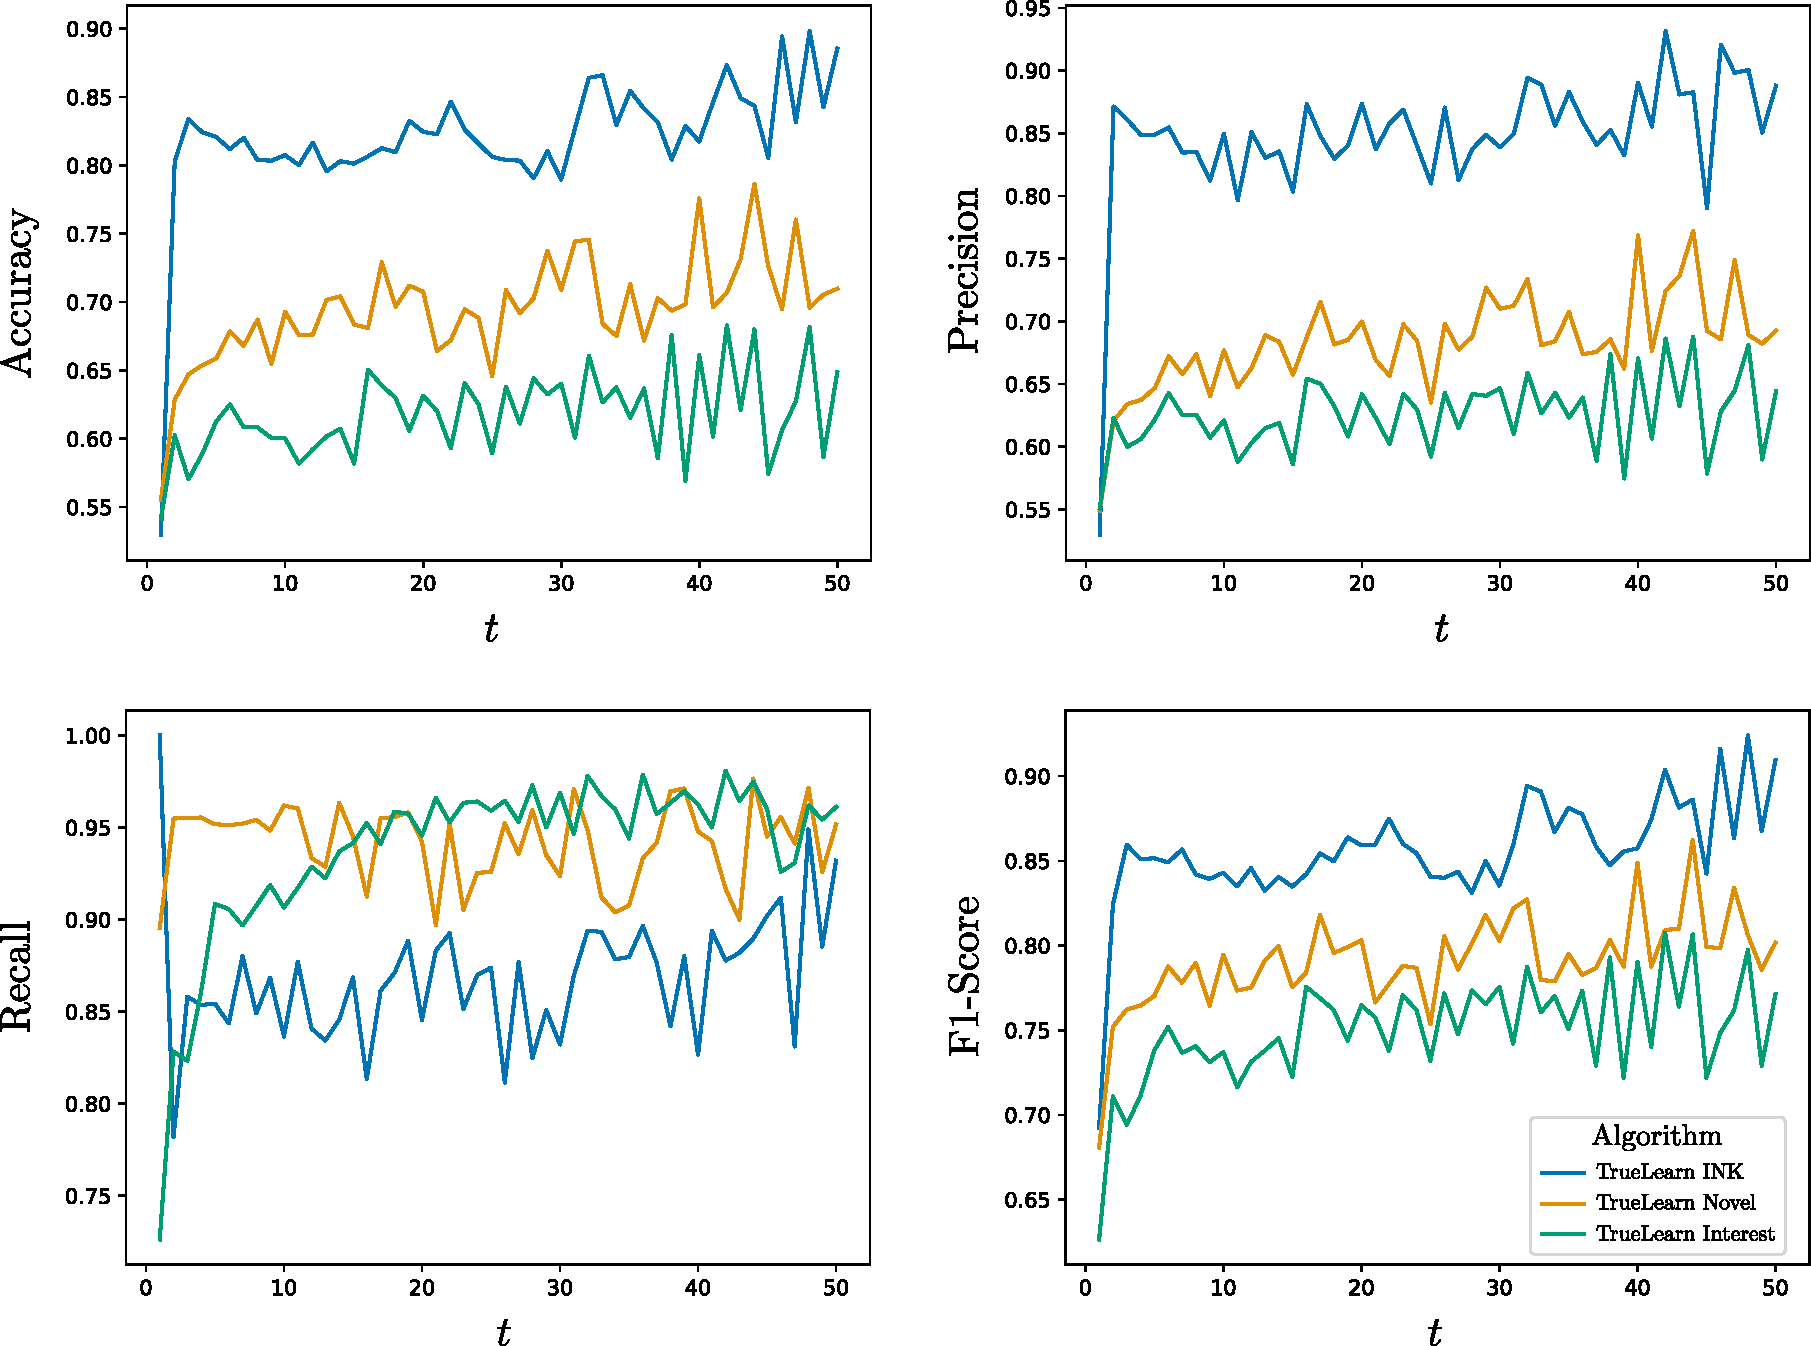
\includegraphics[width=\linewidth]{INK_accuracy.pdf}}
    \caption{How the Mean Accuracy, Precision, Recall and F1-Score at time $t$ across all users in the PEECK test set change on TrueLearn Interest (Green), TrueLearn Novel (Yellow) and TrueLearn INK (Blue) Models across the entire dataset.}
     \label{fig:INK_ACC}
\end{center}
%\vskip -0.2in
\end{figure}

\subsubsection{Improvement of Prediction in the First 10 Events}

Presented in figure \ref{fig:INK_MET}

\begin{figure}[h]
%\vskip 0.2in
\begin{center}
    \centerline{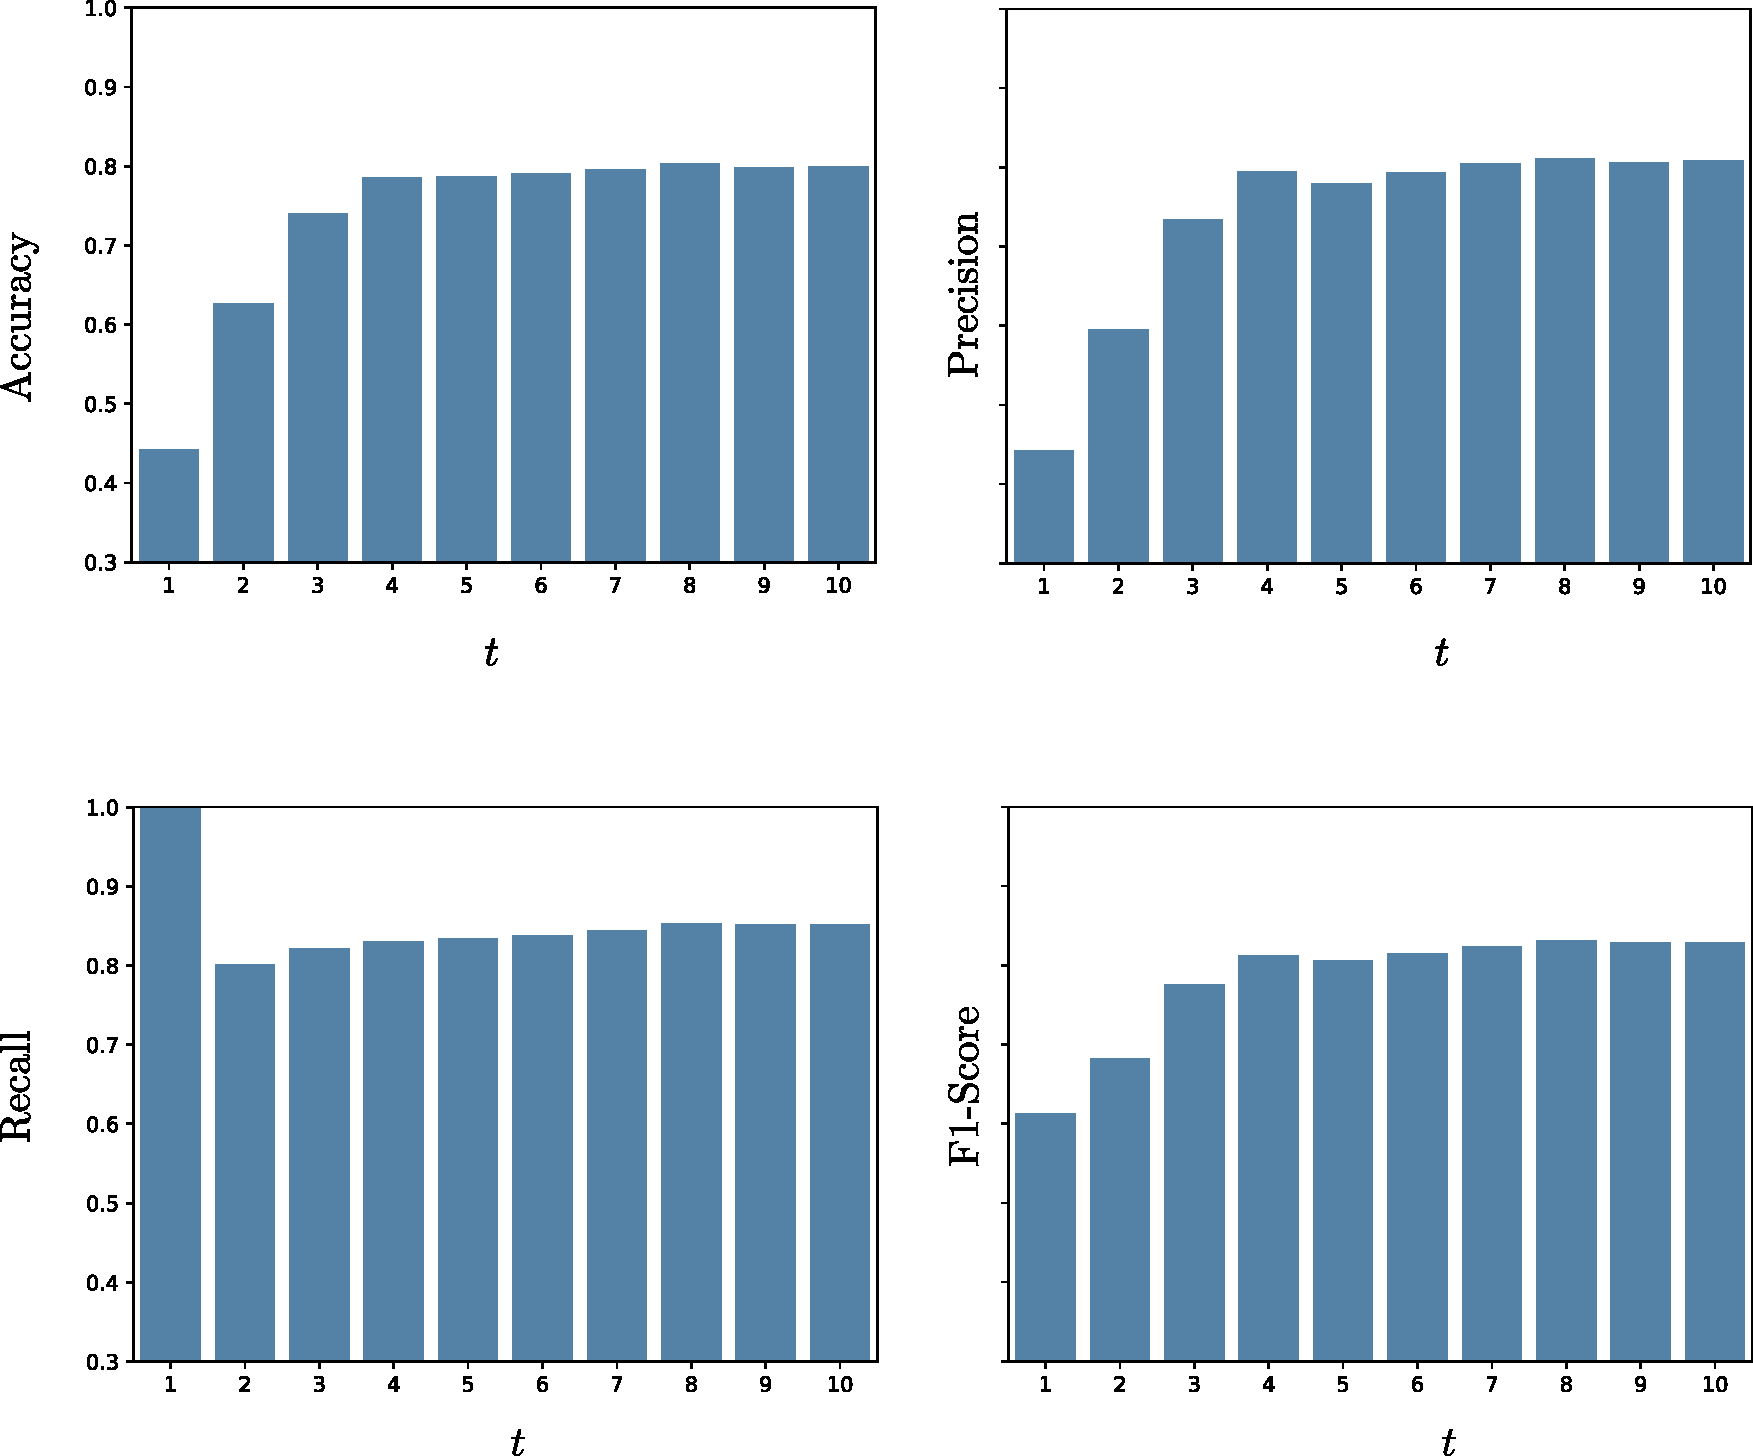
\includegraphics[width=\linewidth]{ink_metrics.pdf}}
    \caption{How the mean Accuracy, Precision, Recall and F1-Score at time $t$ across all the users in the PEEKC test set change the TrueLearn INK Model within the first 10 events.}
    \label{fig:INK_MET}
\end{center}
%\vskip -0.2in
\end{figure}

% \newpage

\subsubsection{Subset of Learner State Visualisations}
\begin{figure}[h!]
%\vskip 0.2in
\begin{center}
    \centerline{\includegraphics[width=\linewidth]{vis_plots.pdf}}
    \caption{A subset of the multiple visualisations available in the TrueLearn library to present the learner state in a humanly intuitive way.}
\end{center}
%\vskip -0.2in
\end{figure}

% \newpage
\subsection{TrueLearn Models}

\begin{figure*}[h]
% \vskip 0.2in
\begin{center}
\centerline{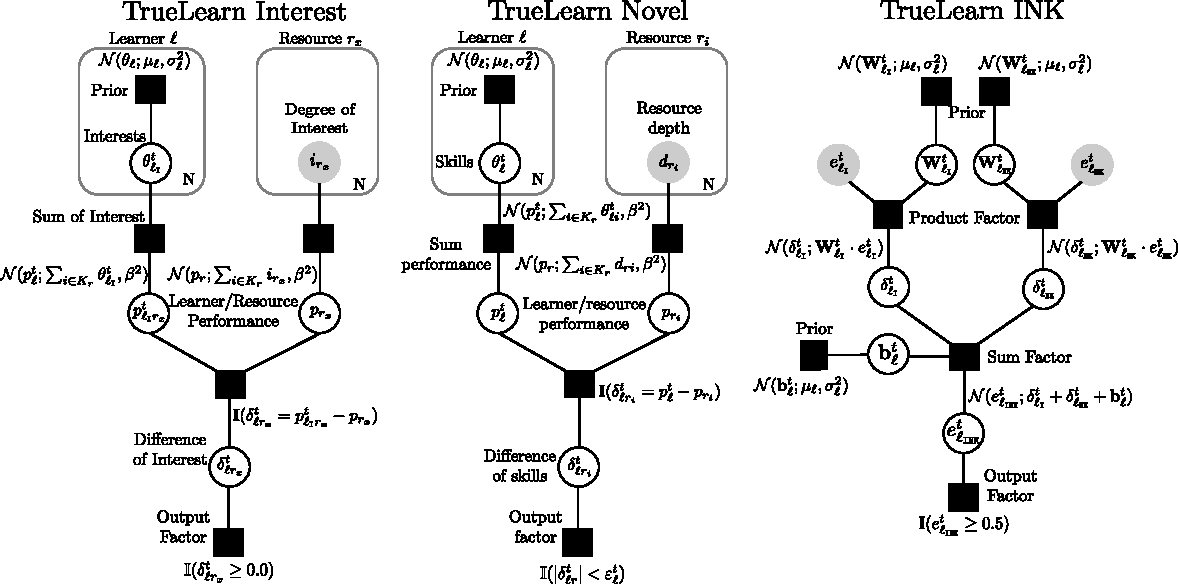
\includegraphics[width=.75\linewidth]{TrueLearn_models.pdf}}
\caption{Factor graphs representing the probabilistic graphical models for TrueLearn Interest (left), TrueLearn Novelty (middle) and TrueLearn INK (right) models.}
\end{center}
% \vskip -0.2in
\end{figure*}



% \newpage
\subsection{Detailed Descriptions of the Columns in the PEEKC Dataset}

Detailed descriptions of the columns in the PEEKC dataset are found in table \ref{tab:features}
\begin{table*}[h] \small
\caption{Detailed descriptions of the different columns of the \texttt{train.csv} and \texttt{test.csv} files included in the PEEKC Dataset.}
\label{tab:features}
\centering
\begin{tabular}{ccl}
\hline
Column Number & Description & Details \\
\hline
1 & Video Lecture ID & An integer ID associated with an individual video lecture \\
2 & Video ID & An integer ID associated to every video belonging to the\\
& & same Video lecture ID (e.g. $1\dots v$ if the lecture has $v$ videos) \\
3 & Part ID & An integer ID associated with each video fragment \\
& & (e.g $1 \dots f$ for a video with $f$ fragments) \\
4 & Timestamp & Timestamp (to the nearest second) when the play event was \\
& &  initiated. \\
5 & user ID & An integer ID associated with each unique learner in the \\
& & dataset PEEKC dataset (IDs in \texttt{train.csv} and \texttt{test.csv} \\
& & files are mutually exclusive). \\
6,8,10,12,14 & KC IDs & An integer ID associated with each unique Knowledge \\
& & Component. This ID can be linked to the human-readable   \\
& & Wikipedia concept names \\
7,9,11,13,15 & Topic Coverage & Proxy for coverage of the relevant KC in the fragment of  \\
& & interest. KC coverage is the cosine similarity. \\
16 & Label & The binary label $e^t_{\ell,r_i}$, 1 if the learner watched $\geq$ .75 \\
& & of the video  fragment, 0 otherwise.\\
\hline
\end{tabular}
\end{table*}

\end{document}